
\documentclass{article}
\usepackage[utf8]{inputenc}
\usepackage{gensymb}
\usepackage{physics}
\usepackage{enumitem}
\usepackage{listings}
\usepackage[margin=0.5in]{geometry}
\usepackage{graphicx}
\usepackage{float}
\graphicspath{ {Images/} }
\usepackage{amsmath}
\newcommand{\tens}[1]{%
  \mathbin{\mathop{\otimes}\displaylimits_{#1}}%
}
%\usepackage[final]{pdfpages}


%\usepackage[spanish]{babel}    
\usepackage[T1]{fontenc}
\usepackage{natbib}
%\usepackage{array}
%\usepackage{gensymb}
\usepackage{indentfirst}
%\usepackage[table,xcdraw]{xcolor}



\title{Optical Pumping Lab}
\author{Joshua Levy\\Lab Partner: Alex Chuang}
\date{UC Berkeley Physics 111B\\March 2017}


\begin{document}

\maketitle

\section{PreLab and MidLab Sign Offs}
\begin{center}
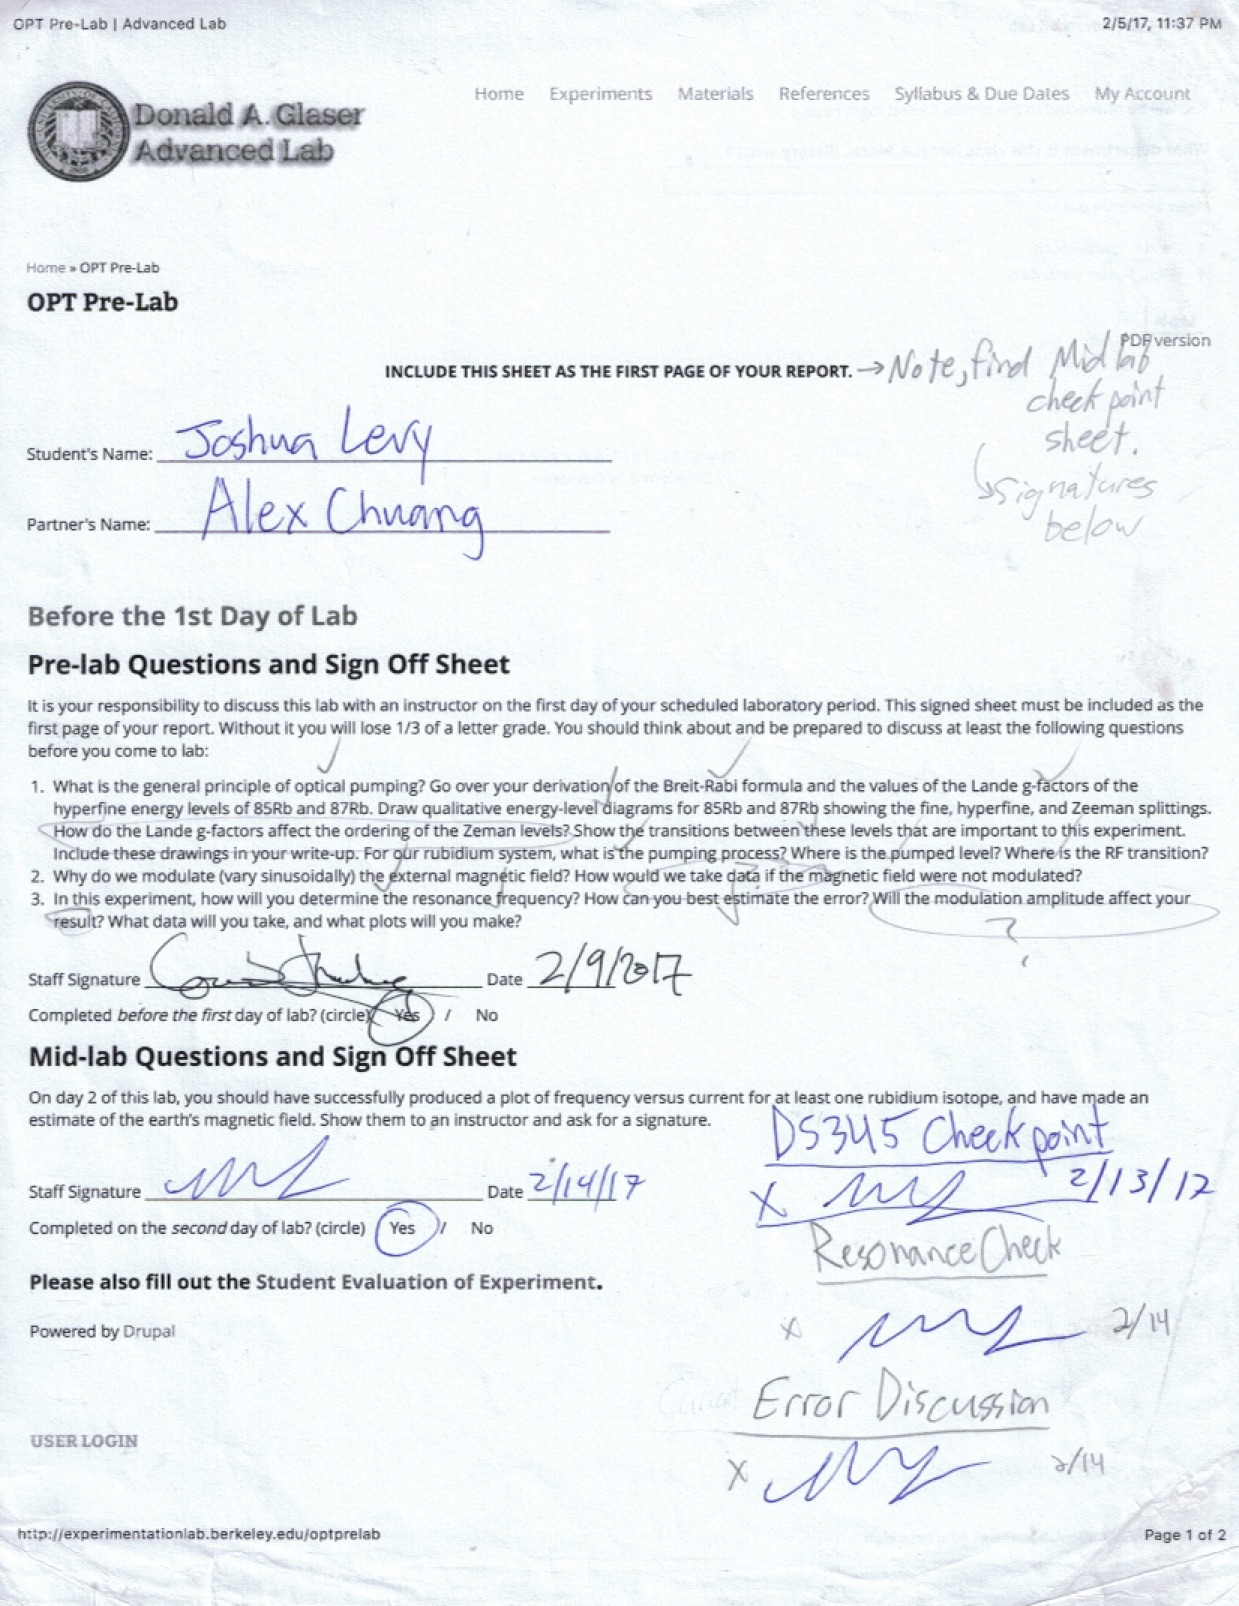
\includegraphics[scale = 0.32]{prelabOPT.jpg}
\end{center}

\newpage


\section{Abstract}
    My partner and I applied circularly polarized light, a modulating externally applied magnetic field and RF frequency light to a gas sample of rubidium to produce the optical pumping effect, where the distribution of lower energy states of rubidium is "pumped" to higher energy levels. By observing the light passing through the gas sample, and using the Breit-Rabi law, we were able to measure the nuclear spins $I_1$ and $I_2$ of two isotopes of rubidium ($^{85}Rb$ and $^{87}Rb$ respectively), for given positive and negative polarities of the externally applied magnetic field. The spin values were found to be $\frac{5}{2}$ for $^{85}Rb$ and $\frac{3}{2}$ for $^{87}Rb$, and were found in moderate agreement with multiple measures. We also used this effect to find the earth's magnetic field for 85Rb and 87Rb in the positive polarity case to be 0.4462 $\pm$ 0.0250 gauss and 0.4502 $\pm$ 0.0040 gauss respectively, and in the reverse polarity case to be 0.4032 $\pm$ 0.0300 gauss and 0.3670 $\pm$ 0.0083 gauss respectively. These field values show moderate agreement with each other. We demonstrated a positive correlation between temperature and signal strength $^{85}Rb$ over the 32 to 45 $\degree$C temperature range, found a zero-field resonance point at -0.0936 amps, and found the pumping and relaxation times for $^{85}Rb$ to be $\tau_p \approx 0.819$ seconds and $\tau_R \approx 0.374$ seconds with 95$\%$ confidence intervals of [0.742, 0.897] and [0.315, 0.433] seconds respectively.


\section{Introduction}
    In this experiment, my partner and I got to witness "quantum mechanics in action". We directly witnessed the effects of fine splitting, hyperfine splitting, and Zeeman effect splittings on a gas sample of $^{85}Rb$ and $^{87}Rb$ Rubidium isotope gas samples through the use of optical pumping.
    \\\indent In the field of quantum mechanics, we can come to the understanding that particles in a bound system have discretized energies. Light of a certain frequency is emitted when the energy of a particle jumps from a higher energy to a lower energy and absorption occurs when the jump is from low to high energy, and the particle becomes excited. As such, light we see is discretized as well. The energy levels that we see for a particular atomic system result from many different atomic effects. The energy levels that we originally find for a system results from a hamiltonian describing kinetic and potential energies. However, these energy levels are "perturbed" when we consider nonclassical effects or generate any fields that introduce more energy in the system. Once degenerate energy levels split into a myriad of different energy levels that are slightly different from the original. On the baseline, we can construct an energy level diagram by considering the discretized energies that result from the coloumb interactions between the orbiting electrons and the nucleus, and the interactions between electrons. Each of these energy levels first undergos fine-structure splitting, where each energy level splits due to relativistic corrections to the kinetic energy of the system, the spin orbit coupling of an orbiting electron (interaction between the magnetic field generated by the orbital angular momentum of the electron with the magnetic dipole moment generated from the electron's spin), and other corrections due to small order expansions of the Dirac equation \cite{fs}.
    These energy corrections are found using perturbation theory. However, after these splittings, the levels are split once more due to smaller order hyperfine structure splitting corrections, taking into account the interaction between the magnetic moments/fields resulting from the spin of the atom's nucleus and from the spin of the electron (these are degenerate perturbations). All of the splittings introduced thus far are a result of effects internal to the atomic system. Furthermore, in this experiment, we introduced external Zeeman splittings, which splits energy levels due to the interaction between an externally applied magnetic field and the magnetic dipole moment of the atomic system. We normally expect to see light (or notice the absence of light) of a certain frequency due to an energy transitions described by $\Delta E = hf$ where f is the frequency. However, the frequencies of observed light change ever so slightly with the introduction of these perturbations. 
    \\\indent We can observe all of these splitting effects by using the optical pumping technique. After generating Zeeman splittings from an externally applied magnetic field, we send circularly polarized light with known angular momentum to be absorbed by a Rubidium sample. This absorption causes a transition from the ground state to an excited state of higher orbital angular momentum and z-component total angular momentum. Due to selection rules and spontaneous emission, the light is reemitted as the energy of the system loses quantized orbital angular momentum, though with no preference towards how much z-component total angular momentum it loses. This favors transitions that will leave the atomic system in a pumped up state, that is, eventually all atoms will be at a state that is the highest energy level of the Zeeman splitting of degenerate level of the ground state. Due to the saturation of optical electrons at this energy level, no more light can be absorbed, and the quantum state is "pumped". We can undo this pumping by applying light (which we call RF, resonance frequency, modulation) to the at such a frequency as to cause the electron to jump again towards its original ground state through stimulated emission. Another way to undo the pumping is to vary magnitude of the Zeeman energy splittings (external magnetic field) so that it matches the frequency of the applied light. By time-varying either the applied magnetic field about a fixed field value or the frequency of the applied light about a purported point of resonance (where absorption and emission occur in a very sinusoidal manner), while keeping the other fixed, we can easily discover the point of resonance for the system. The point of resonance in a system can be described by the total magnetic field at resonance, which can be measured, and the RF light frequency, of which we know because it is input to the system using a function generator. 
    \\\indent In our experiment, we will find all such points for $^{85}Rb$ and $^{87}Rb$ Rubidium isotope gas, plot them, and fit lines through the points to deduce the value of Earth's magnetic field, to find the spin angular momentum values of each nuclear isotope of Rubidium, and to confirm the derivation of the Breit-Rabi formula. The experiment gives us first-had knowledge of what it is like to precisely measure energy levels of atomic systems. Furthermore, we also will explore the effects of the temperature variation of the optical signal's intensity %FIX!!! 
    at resonance, find the Zero Field resonance (resonance point when our RF light source is shut off), and we also will measure the pumping and relaxation time of the system at resonance with square wave amplitude modulation of the RF light. 

    

\section{Theory}
    We can estimate the energy splittings of the atomic system by using time independent nondegenerate and degenerate perturbation theory. A quantum system can be described by a hamiltonian H and its associated energy eigenvector (also using linearity):
    \begin{equation}
        H \ket{\psi} = \sum_ic_i*H\ket{\psi_i} = \sum_ic_i*E_i\ket{\psi_i}
    \end{equation}
    where $\ket{\psi}$ is the energy eigenstate (probability amplitude) to describe quantum state, $\ket{\psi_i}$ is the ith component of it, an energy eigenstate for the energy level $E_i$ that is obtained by operating the Hamiltonian on the eigenstate, and $c_i$ is the orthogonal projection of $\ket{\psi}$ onto its decomposed eigenstate $\ket{\psi_i}$. However, we cannot directly find $\ket{\psi_i}$ due to the complexities of the corrections and the new potentials applied to the system. The system's original Hamiltonian, $H_o$, describes the energy of the system without any interaction effects:
    \begin{equation}
        H_o = T + V
    \end{equation}
    where T is the kinetic energy of the electron and V is the potential energy of the electron inside the atom. If we apply $H_o$ to an quantum state described by quantum numbers n (principle quantum number) and l (orbital angular momentum), we get a returned energy level:
    \begin{equation}
        H_o\ket{nl} = E_{nl}\ket{nl}
    \end{equation}
    where $E_{nl}$ is the returned energy (not to be detailed in this analysis).
    Here, we can neglect or include the Coulomb interaction between the optical electron and the ground state electron (derivation not included). The fine structure of the system can be treated as a perturbation to the Hamiltonian:
    \begin{equation}
        H = H_o + H_{fs}' = H_o + H_r' + H_{so}'
    \end{equation}
    where $H_r'$ is a relativistic correction and $H_{so}'$ is the spin-orbit correction (interaction between spin and orbital angular momentum of the electron). We see:
    %Griffiths
    \begin{equation}
        H_r' = \frac{-p^4}{8m^3c^2},H_{so}' = -\vec{\mu_{S}} \cdot \vec{B_{nucleus}} = (\frac{Zg_se^2}{8\pi\epsilon_o})\frac{\vec{L}\cdot\vec{S}}{m^2c^2r^3}
    \end{equation}%fix
    where p is momentum, m is mass, c is the speed of light, Z is the number of protons in the nucleus, $g_s$ is the spin g-factor, e is electron charge, S and L are spin and orbital angular momentum.%FIX describe all of the terms
    $H_r'$ is found from rearranging the Hamiltonian that includes relativistic correction: $H = \sqrt{p^2c^2 + m^2c^4} - mc^2 + V$. $H_{so}'$ is found by considering the energy of an interaction between the magnetic field generated by the nucleus with the dipole moment from the electron's spin. \\\indent To find the perturbed energy levels $H_r'$, we use nondegenerate perturbation theory choosing the states $\ket{nlm_l}$ ($m_l$ being the z-component of orbital angular momentum) and basis transformations L and $L_z$ to find a first order correction for the hamiltonian:
    \begin{equation}
        E_{r}^1 = \bra{nlm}H_r'\ket{nlm} = -\frac{E_{nl}^2}{2mc^2}(\frac{4n}{l+0.5} - 3)
    \end{equation}
    We find a first order correction for $H_{so}'$ using degenerate perturbation theory, choosing to use basis states $\ket{nljm_j}$ (j is the total angular momentum, and $m_j$ is its z-component) and basis transformations $L^2,S^2,J^2,J_z$. Using the identity $J^2 = S^2 + L^2 + 2\vec{L}\cdot\vec{S}$, and applying the perturbed hamiltonian, we find this correction to be:
    \begin{equation}
        E_{so}^1 = \bra{nljm_j}H_{so}'\ket{nljm_j} = \frac{E_{nl}^2}{mc^2}*\frac{n[j(j+1) - l(l+1)-0.75]}{l(l+0.5)(l+1)}
    \end{equation}
    In this analysis we neglect the effect from Dirac's Equation. We denote such a Hamiltonian to be $H_1$:
    \begin{equation}
        H_1 = H_o + H_{fs}'
    \end{equation}
    The remaining splittings used in this experiment are hyperfine splittings ($H_{hfs}'$) and Zeeman effect splittings ($H_{hfs}'
H_{Z}'$). The hyperfine splitting is small relative to the fine splitting. We assumed that the magnetic field produced is of small magnitude, and that any splitting arising from the field can be treated as a perturbation to the hyperfine splitting. In real life, the assumption we made about the magnetic field is not true, so we cannot truly treat the zeeman splitting as a perturbation. So the final Hamiltonian we wish to consider is:
    \begin{equation}
        H = H_1 + H'' = H_1 + H_{hfs}' + H_{Z}'
    \end{equation}
    where:
    \begin{equation}
        H_{hfs}' = -\vec{\mu_I}\cdot(\vec{B_{nucleus}}) = a*\vec{I}\cdot\vec{J}, H_{Z}' = -(\vec{\mu_I} + \vec{\mu_J})\cdot\vec{B_{ext}} = -(\frac{\mu_J}{J}\vec{J} + \frac{\mu_I}{I}\vec{I})\cdot\vec{B_{ext}}
    \end{equation}
    $B_{ext}$ is our external magnetic field, $a$ is a proportionality constant (will not go into great detail), and $\vec{\mu_I}$ is the magnetic dipole moment resulting from the nuclear spin $\vec{I}$, and the magnetic field at the nucleus $B_{nucleus}$ results in $\vec{J}$ interacting with $\vec{I}$. $\mu_J$ is the magnetic moment resulting from the total angular momentum of the orbiting electron. We can describe eigenstates of $H_{hfs}'$ using the quantum numbers F and $m_F$ (z-component), where 
    \begin{equation}
        \vec{F} = \vec{I} + \vec{J}
    \end{equation}
    Basis states can be described as $\ket{Fm_F}$. Treating $H_{Z}'$ as a perturbation to $H_{hfs}'$, we find that the same basis, $\ket{Fm_F}$, can be used to describe first order Zeeman corrections to the hyperfine splittings. Utilizing the above equation with the three relations $I^2 = F^2 + J^2 - 2\vec{J}\cdot\vec{F}$, $\vec{J}\cdot\vec{F} = \frac{F^2 + J^2 - I^2}{2}$, and $F^2 = I^2 + J^2 + 2\vec{I}\cdot\vec{J}$, and supposing $\vec{B_{ext}}$ to be pointing in the z-direction, we find the first order energy corrections of H$''$ to be:
    \begin{equation}
    \begin{array}{cc}
        W(F,m_F) = \bra{Fm_F}H''\ket{Fm_F} = \bra{Fm_F}a*\vec{I}\cdot\vec{J}-(\frac{\mu_J}{J}\vec{J} + \frac{\mu_I}{I}\vec{I})\cdot\vec{B_{ext}}\ket{Fm_F}\\ = \frac{a[F(F+1) - I(I+1) - J(J+1)]}{2} - \frac{\mu_J[F(F+1) + J(J+1)-I(I+1)]*m_F*B_{ext}}{J*2F(F+1)}
        \end{array}
    \end{equation}
    For this experiment, we consider the case that J = $\frac{1}{2}$, and after some rearrangement/plugging in to the above equation we find that an energy transition ($\Delta W = hf$) between states yields a frequency f of light emitted/absorbed:
    \begin{equation}
        \frac{f}{B_{ext}} = \frac{2.799}{2I+1}
    \end{equation}
    which is the Breit-Rabi law in the low field case, in units MHz/gauss. The g-factor associated with the split hyperfine states are:
    \begin{equation}
        g_J \approx \frac{3}{2} + \frac{S(S+1) - L(L+1)}{2J(J+1)}, g_F = g_J*\frac{F(F+1) - I(I+1) + J(J+1)}{2F(F+1)}
    \end{equation}
    and we could plug in the case where J = S = $\frac{1}{2}$, and the g-factors are used to help find the Breit-Rabi law, and are more intimately involved with describing particular magnetic dipole moments of the nucleus and orbital electron. In this experiment, we will be studying the 85-Rb and 87-Rb isotopes of Rubidium. In this experiment, J = $\frac{1}{2}$ for 85-Rb and J = $\frac{3}{2}$ for 87-Rb, and for 85-Rb, the nuclear spin I is $\frac{5}{2}$, and for 87-Rb, I = $\frac{3}{2}$, and we can find associated g-factors. We see that for the relation in eq.(11), %FIX 
    that the possible values for F are I$\pm \frac{1}{2}$ ($I-J\leq F \leq I + J$), which we can apply to each I value above.
    \\\indent To summarize the previous discussion on energy splittings, we can look at the qualitative energy splitting diagrams below for the case of 85-Rb and 87-Rb:
    \begin{figure}[H] %FIX
        \centering
        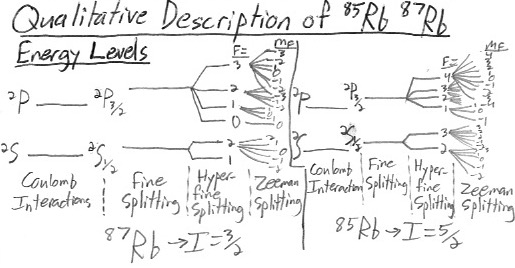
\includegraphics[scale = 0.4]{11.jpg}
        \caption{Some Energy Splittings of 85-Rb and 87-Rb}
        \label{fig:my_label}
    \end{figure}
    We see that the energies of from the Coulomb interaction are split and offset after considering the fine structure interactions/couplings (special relativity and spin-orbit coupling). These degenerate splittings further split due to hyperfine coupling (interaction between the nuclear magnetic dipole moment and the magnetic field found at the nucleus), which are then further split due to Zeeman interactions (interaction between the electronic and nuclear magnetic moments and an externally applied magnetic field, coming from the Earth's magnetic field and an experimentalist applied field). Each time a splitting occurs, the magnitude of it decreases.
    \\\indent We will investigate these splittings, find the nuclear spins of the 85-Rb and 87-Rb and determine Earth's magnetic field by using optical pumping. We will be placing Rubidium atoms into a magnetic field and sending in circularly polarized light to cause absorption (energy transition between the Zeeman levels) in the Rubidium atoms. The selection rules for circularly polarized light dictates that the transition is $\Delta m_F = +1$, $\Delta j = \pm1,0$ and $\Delta l = \pm1$. We will use the figure below describing the energy transitions in 85-Rb to illustrate the point we are about to make. 
    \begin{figure}[H] %FIX
        \centering
        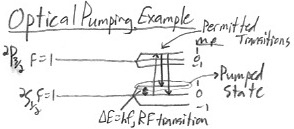
\includegraphics[scale = 0.5]{13.jpg}
        \caption{Example of Optical Pumping Transitions, RF frequency Transition and Pumped State}
        \label{fig:my_label}
    \end{figure}
    \indent In the figure we see that the electron is in a $^2S_{\frac{1}{2}}$ (l=0) state ($\ket{F=1,m_F = 0}$), which we consider the ground state of the hyperfine/Zeeman splittings (though this is not the exact ground state of the splittings). The circularly polarized light is absorbed, and the optical electron jumps to an $\ket{l=1,F=1,m_F=1}$ state. Then, the electron, due to spontaneous emission, emits a linearly polarized photon and experiences a transition with $\Delta l = -1, \Delta m_F = 0,-1$, and the state drops to $\ket{l=0,F=1,m_F=0}$ or $\ket{l=0,F=1,m_F=1}$ (in the real Rb atom, there exists pumping to a few different quantum levels). We see that in this example that the spontaneous emission causes the electron to drop into those two possible states, the emphasis is that it does not really favor one particular state in the transition (the probability of transitions are a bit different, but the important part is that it has a chance of transitioning to either lower energy level). As such, we also know due to selection rules, that a state sitting in $\ket{l=0,F=1,m_F=1}$ cannot undergo absorption, so it will stay in that state if a photon enters the system. However, the remaining $\ket{l=0,F=1,m_F=0}$ quantum states can undergo this absorption, so by repeating this process, we distribution of quantum states is "pumped" from the ground state ($\ket{l=0,F=1,m_F=0}$) to the "pumped" state $\ket{l=0,F=1,m_F=1}$ (i.e. some distribution of quantum states throughout our Rb gas sample becomes concentrated at a higher quantum level in the Zeeman split energy levels). On the diagram we have marked the transitions that can occur in this example, and where the pumped and ground energy levels are. We see that when most of the particles in the system are pumped to this pumped state, then the gas can no longer absorb more light, and if we were to use a detector to measure the signal of the total light passing through the sample, we would see that over time, as we begin pumping, that the signal of light would have a low amplitude when absorption is high, then the amplitude would increase and asymptote as the quantum states are pumped. However, if we apply RF light with energy $\Delta E$ = hf to the pumped quantum states, the magnitude of this energy being equal to the energy spacing between $\ket{l=0,F=1,m_F=0}$ and $\ket{l=0,F=1,m_F=1}$, we can cause the stimulated emission of a photon of the same energy, and cause the pumped up state to transition to the specified lower state (an R-F transition, marked in the above figure), thereby allowing the sample of gas to begin absorbing circularly polarized light again. In the introduction, we mentioned that varying either the Zeeman splittings through the applied magnetic field or the RF-frequency while keeping the other fixed will allow us to find the point of resonance, where the RF-transition energy is equal to the spacing between the ground and pumped energy levels.
    \\\indent In this experiment, we modulate the magnetic field B(t) about a fixed magnetic field value $B_o$ to establish a point of resonance (we also sweep through RF frequencies in the beginning of the experiment, but it was not the most useful for our analysis, so we leave the RF-frequency fixed). As we time-vary the externally applied magnetic field, we change the offset of this field such that the Zeeman splittings it produces can have the same energy magnitude as the RF-transition at a point in time during the oscillation (in this sense we have measured the Zeeman spacings). We use the five diagrams below to illustrate this concept: 
    \begin{figure}[H] %FIX
        \centering
        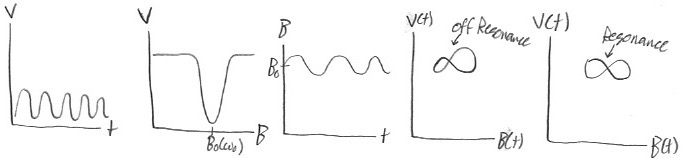
\includegraphics[scale = 0.4]{16.jpg}
        \caption{Plots of Light Signal V found at photo detector, static magnetic field B, modulated B field B(t), versus time; including lemniscate figure}
        \label{fig:my_label}
    \end{figure}
    \indent We represent the light signal passing through the gas sample (a voltage measured through a detector) as V(t). If we plotted the magnetic field with no modulation versus V, we see that there is a magnitude of the B field by which the pumped states are relaxed, where we see the most absorption (global minimum). As we time-vary this magnetic field, we oscillate about this global minimum, and we see that if we where to plot V versus time, that the signal would oscillate as the states are pumped and then unpumped (we see an oscillatory cycle between emission/light passing through and absorption). If we plot the modulated magnetic field B(t) versus the signal V(t), we see that near the point of resonance, it produces this geometric shape seen above. If the shape is asymmetrical, then our modulated magnetic field is not oscillating about the proper fixed magnetic field value that produces the Zeeman splitting spacings that are the same as the RF-frequency (the asymmetry is produced because instead of oscillating about the global minimum in the graph of static B versus V, we oscillate off center). We adjust the offset of the magnetic field until the shape becomes symmetric, and then we know that this point ($B_o,f$) describes resonance and the Zeeman energy spacing including the fine structure and hyperfine structure interactions. We can reexpress eq.(12) %FIX
    as:
    \begin{equation}
        f = \frac{2.799}{2I+1}*(B_E + B_o)
    \end{equation}
    with $B_E$ being Earth's magnetic field. For Rb-85 (I=$\frac{3}{2}$) and Rb-87 (I=$\frac{5}{2}$), we can fit found data points to a line, where we can use the slope to help find the nuclear spin values of both isotopes, and the intercept to help find the value for Earth's magnetic field. The magnetic field was generated by passing current through Helmholtz coils, and we assumed the field at the center of the Rubidium bulb to be:
    \begin{equation}
        B_o = \lambda*\frac{Ni}{A}
    \end{equation}
    where N is the total number of turns in the coils, i is the current passing though the coil (which we will measure during the experiment to estimate the resonance field $B_o$), A is the radius of the coil loop, and $\lambda$ is the constant $0.9*10^{-6}$ ($\frac{tesla*meter}{ampere}$).\cite{opt} 
    \\\indent During the experiment, we will be heating up a bulb (by passing electrical current through coiled wires beneath the bulb; heat being generated by the friction of electron interactions) filled with rubidium in order to release rubidium atoms off the walls of the bulb and into the gas in the center of the bulb. The rubidium atoms on the walls of the bulb will experience the heterogeneous magnetic effects as aforementioned, so it is important to heat up the bulbs as to get closer to our true magnetic field estimate. But when the temperature is too high, the collision rate between neighboring Rb atoms can consequently cause some stimulated emission of the pumped states, thereby causing some attenuation in our signal. We will explore this effect along with other temperature effects and note how the temperature of the bulb effects our signal strength and relative changes in our points of resonance.
    \\\indent The last effect we will explore during this experiment is the optical pumping and relaxation time. By modulating our RF-frequency light (of a fixed frequency) (already set to resonance/absorption with the magnetic field) with a square wave, we can turn on and off pumping in a periodic fashion and observe the light signal that passes through (V).
    \\\indent After accounting for any offset arising from the minimum signal of V, we will measure the time it takes for the signal to reach $1-\frac{1}{e}$ times the signal's maximum value during the pumping stage right after relaxation (pumping time). Then when the square modulation is low, we will measure the time it takes for the signal to decrease from its maximum value down to $\frac{1}{e}$ times its maximum value (relaxation time). The details of this calculation will be included in the calculations section.
    \\\indent In this lab we assume that the helmholtz magnetic field is constant at the center of the gas sample. However, this is not true. The field is heterogeneous in magnitude and direction, especially at the boundaries of the rubidium bulb, somewhat due to the nonzero width windings of the coils and the spacial differences in the field near the center. Such effects, along with the introduction of stray magnetic fields, may cause the magnetic dipole of the quantum state to become misaligned with the total magnetic field, causing transitions to non-pumping states. It is necessary that the helmholtz coils are aligned nearly perfectly with Earth's magnetic field in this case.\cite{nuc}

\section{Apparatus and Procedure}
    \begin{figure}[H] %FIX
        \centering
        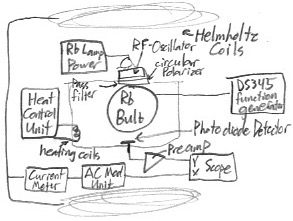
\includegraphics[scale = 0.45]{18.jpg}
        \caption{Diagram of Experimental Apparatus}
        \label{fig:my_label}
    \end{figure}
    The above figure describes our experimental apparatus. Brief descriptions for each major component is listed below:
    \begin{itemize}
        \item Rb Bulb- Contains sample of 85-Rb and 87-Rb isotope gas; the quantum states in the samples will be pumped up due to incoming circularly polarized light and then relaxed due to RF-light at the resonant frequency; also contains inert buffer gas that localizes Rb atoms to keep them within the volume of the bulb and away from the glass walls
        \item Heat Control Unit- Supplies power to coils that heat up the sample, allowing the vaporization of Rb atoms stuck on the walls of the bulb to increase the optical pumping signal; contains a temperature sensor that allows you to see temperature of bulb
        \item Rb Lamp + Power Supply- Current is supplied to lamp that causes light to be emitted towards sample
        \item Circular Polarizer- Circularly polarizes light emitted from the Rb Lamp, such is necessary to cause optical pumping effect
        \item Photodiode detector- Converts an incoming light signal into an electrical signal to be passed on to the oscilloscope; useful for finding out the opacity of the Rb sample during pumping and relaxation
        \item PreAmp (SR560)- Electrical signal from the photodetector is amplified by this device because the original signal from the radiation is very small and needs to become readable. 
        \item Helmholtz Coils + AC Modulation Unit/Coil Driver- Produces externally applied magnetic field that causes Zeeman splittings (assuming field points in z-direction, and points along the cylindrical axis at the center of the coils). A user-specified current is sent in from a power supply, which can be adjusted using the current knob, and it is measured using a $10m\Omega$ shunt (operates like a calibrated resistor). The current reading is measured by a voltmeter, which registers the voltage drop across the shunt, and using these values of resistance and the measured voltage and ohm's law, we can find the current, "i", that is generating the magnetic field (to be used in our calculations). To help find resonance, the field is modulated about this constant field through an AC modulation unit. On this unit, we can specify the polarity of the total current, the modulation amplitude, the phase of the modulated magnetic field, and turning on or off this modulation can be specified. 
        \item DS345 Function Generator- This device generates modulated signals of the user's specification to be output to the RF-oscillator, where the signal is coverted into an RF-light signal. The signal produced here essentially generates the light signal that will go into the Rb sample to cause stimulated emission and thus relaxation of the pumped energy states. In this experiment we will be sweeping various frequencies when testing for our initial resonance points.
        \item Oscilloscope- The outputs from the magnetic field modulation unit and the photodetector (after amplification from the preamp) will be input into this device that measures input signals over time. We can measure the two inputs separately over time or we can plot the two together. In this experiment we will input signals from other apparatus components as well.
    \end{itemize}
    For the SR560, DS345, and the oscilloscope, please read their equipment manuals to understand which settings to use for a useful and safe setup. Do not let the temperature of the Rb Bulb exceed 55$\degree$C (we did this by turning on and off the heating coils to maintain a near constant temperature in the sample; the coils were turned off during recording). \\\indent The purpose of the first part of our experiment was to find resonance points and plot them in order to find the nuclear spins of 85-Rb and 87-Rb, to find Earth's magnetic field, and to confirm the Breit-Rabi law in the low field case. First, we turn on all of the aforementioned equipment and set the SR560 preamp to its specified settings, turn on the heating coils (up to 25 milliamps) for the rubidium gas, and turn on the DC power supply to the AC modulation unit and the function generator (producing RF modulation to be fed into the Rb gas). We find the initial points of resonance by first inducing a current through the Helholtz coils to produce Zeeman splittings, the more current applied will produce larger splittings. We are not AC modulating the magnetic field at this point. We connected the modulation to channel 1 of the oscilloscope and the amplified signal (preamp) to channel 2 of the scope, and with the scope set to X-Y mode. After calculating expected resonance points (Breit-Rabi) for 85-Rb and 87-Rb for a given current, we output a sine wave signal and sweeped RF frequencies (using the function generator) $f\in$[$f_{midpoint}-\frac{span}{2},f_{midpoint} + \frac{span}{2}$] (chosen midpoint between the two calculated resonant frequencies with a large span/range) near the expected resonance points to produce the below figure:
    \begin{figure}[H] %FIX
        \centering
        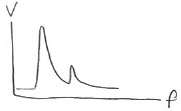
\includegraphics[scale = 0.4]{15.jpg}
        \caption{Frequency Scan Output on Scope; Helps Find Resonance Points}
        \label{fig:my_label}
    \end{figure}
    \indent We see that the peaks in the figure correspond to the resonance frequencies. We increased or decreased the midpoint frequency used in the frequency sweep to center it on one of the two isotopes' resonance frequencies and decreased the span to further center it on a resonance frequency. RF modulation does not provide the most accurate way of finding points of resonance, so once we centered the frequency sweep about a point of resonance, we held the RF frequency constant, replaced channel 1 of the scope with the signal from the AC modulation unit and channel 2 with the signal found from the photodetector (preamp output; B vs. V), and turned on the modulating magnetic field on the AC modulation unit. The modulating magnetic field will oscillate the Zeeman splitting spacing about the energy of the constant resonant frequency RF light. Here, for each found resonance point, we changed the current in the Helmholtz coils to adjust the offset of the magnetic field signal such that the modulated AC component of the field (Zeeman splittings of the field) oscillates about the energy of the RF frequency. We can notice a point of resonance when the output of the oscilloscope in X-Y mode looks like a symmetric and offset (by the B-field voltage across the shunt which measures the current in the Helmholtz coils) lemniscate, as detailed in the theory section. If the shape is not symmetric, then we adjusted the current until the shape becomes symmetric. We aided in this adjustment by looking at channel 2 in the time domain, which is depicted in the figure below:
    \begin{figure}[H] %FIX
        \centering
        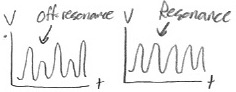
\includegraphics[scale = 0.4]{17.jpg}
        \caption{Time Domain of Channel 2/Light Signal Output}
        \label{fig:my_label}
    \end{figure}
    \indent Ideally, if the B-field is oscillating about a point of resonance, in the time-domain of the photodetector output, we expect to see neighboring peaks of equal height, or else the energy spacing by which the Zeeman splittings are oscillating about is not equal to the energy spacing of the RF transition. We change the current until the two neighboring peaks are equal. However, due to various effects and internal reflections in the equipment, the modulating magnetic field may be slightly out of phase with the signal from the photodetector, so in the X-Y mode of the scope, we adjust the "Phase Adjust" knob of the AC modulating unit and make small changes to the current accordingly to produce a completely symmetric figure translated lemniscate figure (we could center this translation using oscilloscope position adjustments). We record the RF transition frequency by looking at the frequency set by the function generator and find the external magnetic field at resonance by looking at the output of a voltmeter depicting the voltage drop across the shunt, and converting the observed value to a current. Once we have found this single point of resonance, we changed the RF frequency of the function generator, and adjusted the current to find the new resonance point accordingly. For all found resonance points, we held the AC modulation amplitude fixed. After we collected enough points for one isotope, we reversed the polarity of the Helmholtz coils via an option on the AC modulation unit, and collected resonance points for that isotope with negative current values. Finally, we repeated the process for the other rubidium isotope. For each isotope resonance line being produced (two for each polarity of the field), we estimated the error of the current values by changing the modulation amplitude of the AC magnetic field by 10, and recording all resonance currents, given one fixed RF frequency. We then assumed that the error yielded by the variation of datapoints is the same for all resonance points on that particular isotope/polarity line. 
    \indent We found zero field resonance by turning off the RF generator (energy of RF transition reduces to 0J), and then varying the current until we've found a point of resonance (also using reverse polarity magnetic field). We've set the field modulation to 100. We recorded the current at resonance.
    \\\indent We then looked for the variation in the signal strength of the photodetector signal due to temperature effects. We held the modulation frequency fixed, and found a particular point of resonance using the method above. Due to time constraints, we could only do this for 85-Rb in the reverse polarity field case. Using the heat controller, we varied the temperature of the Rb sample in increments between 32$\degree$C to 45$\degree$C, and found the maximum signal of the photodetector output by counting the divisions on the oscilloscope that were between the maximum voltage of the channel 2 and the minimum voltage in X-Y mode (lemniscate figure). The error in the voltage/signal strength was found by counting the divisions of fuzziness (measurement error) in the maximum and minimum voltage points after the image was focused. 
    \indent Finally, we were also able to measure the pumping time at resonance with square wave modulation of the RF light. First, we found the resonance RF frequency when the current applied to the Helmholtz coils was around 1 Amp. Then, using the function generator, we modulated that RF signal using a square wave. Once again, the modulation output from the function generator when to channel 1 of the oscilloscope while the output of the photodetector (after preamp) when to channel 2. We plotted both channel 1 and channel 2 in the time domain with 0.5 seconds/division and used a horizontal magnification of x5. We adjusted our voltage per division accordingly until we would observe the signal oscillate between exponential decay and exponential growth, as depicted in the figure below. We noticed that the timing of these exponential functions closely paralleled the high and low outputs of the RF square modulation output: 
    \\\begin{figure}[H] %FIX
        \centering
        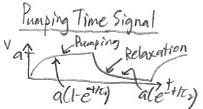
\includegraphics[scale = 0.5]{14.jpg}
        \caption{Qualitative Expected Output of Channel 2 of Scope}
        \label{fig:my_label}
    \end{figure}
    \indent We recorded high speed videos of the processes occurring, and analyzed them for pumping and relaxation times respectively, taking into account any introduced errors. The sample was pumped when the RF modulation was in the high output (exponential decay output), and relaxed when the RF modulation was in the low output (exponential growth function with a decay factor).

\section{Calculation and Data Analysis}
    \indent In the Raw Data section, you can find the resonance points that we have produced through the aforementioned methods (table 3). We plotted four datasets (two for each isotope: positive and reverse current polarity) current (i, Amps) versus RF frequency (f(i), MHz) points on the graph below.
    \begin{figure}[H] %FIX
        \centering
        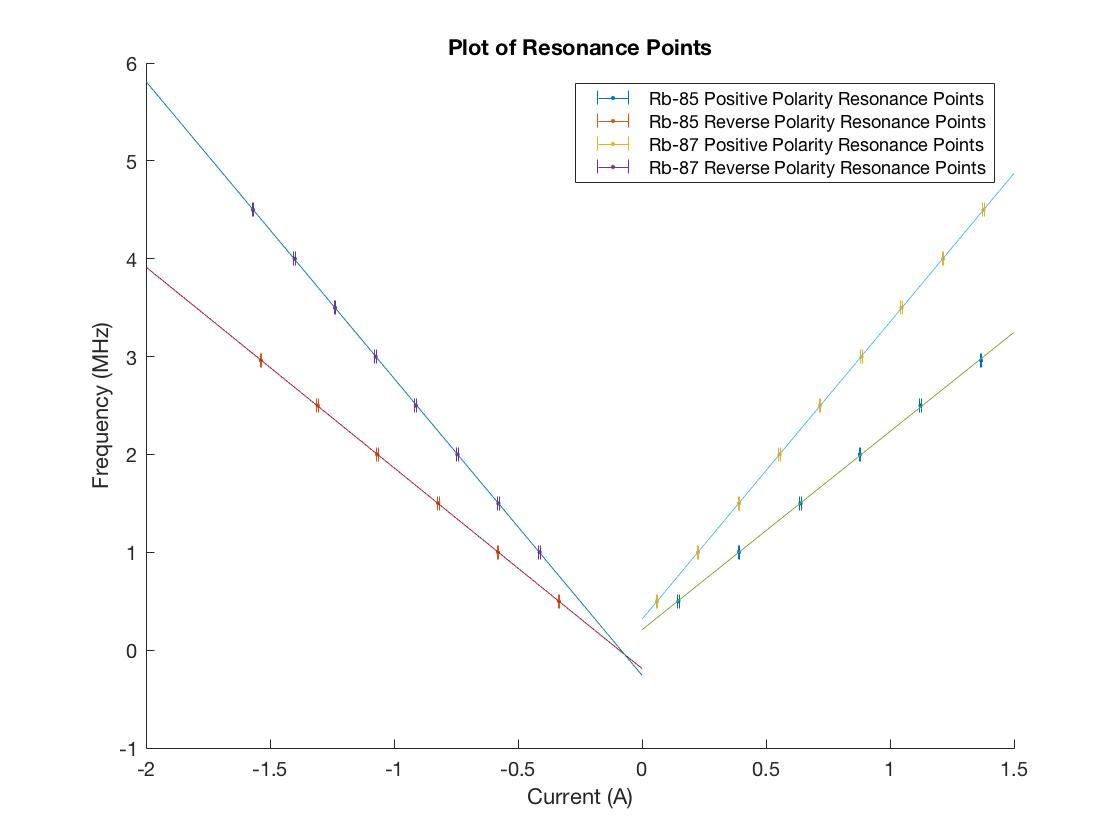
\includegraphics[scale = 0.25]{1.jpg}
        \caption{Plot of Resonance Points for Rb}
        \label{fig:my_label}
    \end{figure}
    \indent We have also included lines of best fit to describe the data in the above graph, and the polarity of the current and the isotopes for each dataset is labelled. We found the best-fit lines for each of the four datasets using a least-squares regression fitting, yielding the function f = m*i + b. From Taylor, we find the slope m and intercept b of N data points \cite{err}:
    \begin{equation}
        m = \frac{\sum_{i=1}^N i_i^2 \sum_{i=1}^N f_i - \sum_{i=1}^N i_i \sum_{i=1}^N i_i*f_i}{\Delta},
        b = \frac{N\sum_{i=1}^N(i_i*f_i) - \sum_{i=1}^N i_i \sum_{i=1}^N f_i}{\Delta}
    \end{equation}
     According to Taylor, the best estimate for the uncertainty in frequency f from the scatter of N data points about the best fit line is:
    \begin{equation}
        \sigma_f = \sqrt{\frac{1}{N-2}\sum_{i=1}^N(f_i-(m*i_i + b))^2}
    \end{equation}
    for found values m and b for a particular fit, and we can calculate the uncertainty in the slope and intercept of each best fit line using the expressions:
    \begin{equation}
        \sigma_m = \sigma_f*\sqrt{\frac{N}{\Delta}},
        \sigma_b = \sigma_f*\sqrt{\frac{\sum_{i} i_i^2}{\Delta}}
    \end{equation}
    where $i_i$ is the ith current measurement and $\Delta$ is:
    \begin{equation}
        \Delta = N*\sum_{i=1}^N i_i^2 - (\sum_{i=1}^N i_i)^2
    \end{equation}
    If we run these calculations (using MATLAB) for each isotope and polarity combination, we get the following fit parameters for f = m*i + b:
    % Table generated by Excel2LaTeX from sheet 'Sheet3'
\begin{table}[H]
  \centering
  \caption{Slope and Intercept of Best Fit Lines for f(i)}
  \scalebox{0.7}{
    \begin{tabular}{lrrrr}
    \textbf{Isotope-Polarity:} & \multicolumn{1}{l}{\textbf{m (MHz/Amp)}} & \multicolumn{1}{l}{\textbf{$\sigma_m$ (MHz/Amp)}} & \multicolumn{1}{l}{\textbf{b (MHz)}} & \multicolumn{1}{l}{\textbf{$\sigma_b$ (MHz)}} \\
    85Rb-Positive & 2.026 & 0.0135 & 0.2081 & 0.0116 \\
    85Rb-Negative & -2.051 & 0.0136 & -0.1881 & 0.0140 \\
    87Rb-Positive & 3.039 & 0.0027 & 0.3150 & 0.0028 \\
    87Rb-Negative & -3.034 & 0.0047 & -0.2568 & 0.0058 \\
    \end{tabular}}%
  \label{tab:addlabel}%
\end{table}%
In this experiment, there are many sources of error and uncertainty, whether it be systematic or measurement errors or other intrinsic uncertainties. For each resonance point (i,f) recorded, there is an associated error $\Delta i$ and $\Delta f$. We found data points describing $\Delta i$ using the method found described in the procedure (Table 4). For each set of data points (resonant current values found from B-field modulation amplitude changes at a fixed RF frequency for given isotope and polarity), we found $\Delta i$ by taking the standard deviation of the data set. This was to account for possible sources of systematic error in our procedure. These errors are much larger than any uncertainties introduced the measurement of the current via the voltmeter, so we disregard errors introduced by the voltmeter. Found values for $\Delta i$ are: \\
\indent Rb-85 Positive: 0.003424 A, Rb-85 Negative: 0.004237 A, Rb-87 Positive: 0.004984 A, Rb-87 Negative: 0.003737 A
\\$\Delta f = 1 \mu Hz$, and is given by the frequency resolution of the DS345 Function Generator \cite{function}.
We consider the order of this frequency resolution ($\mu Hz$) negligible compared to the order of the frequencies we are measuring (MHz), so we can ignore this error.
\\\indent We can see how good of a fit our model f = m*i + b is by performing reduced Chi-Squared values and $R^2$ correlational coefficient values (describes what percent of the data can be described by the best fit model, a measure of how well the best fit line approximates real data points). However, for each of the four models, we are considering an error $\Delta i$ for each data point. Thus, this requires us to invert function that describes our model. We invert f(i) = m*i + b (either directly inverting or exchanging i and f in the above fit parameter calculations) to find i(f) = $m'$*f + $b'$. For each data set, we have now plotted resonance points described by frequency versus current and also have made a residual plot for the data (each ith residual point is calculated from $i_{observed} - i(f_{observed})$). The data along with best fit lines have been plotted below:
\begin{figure}[H] %FIX
        \centering
        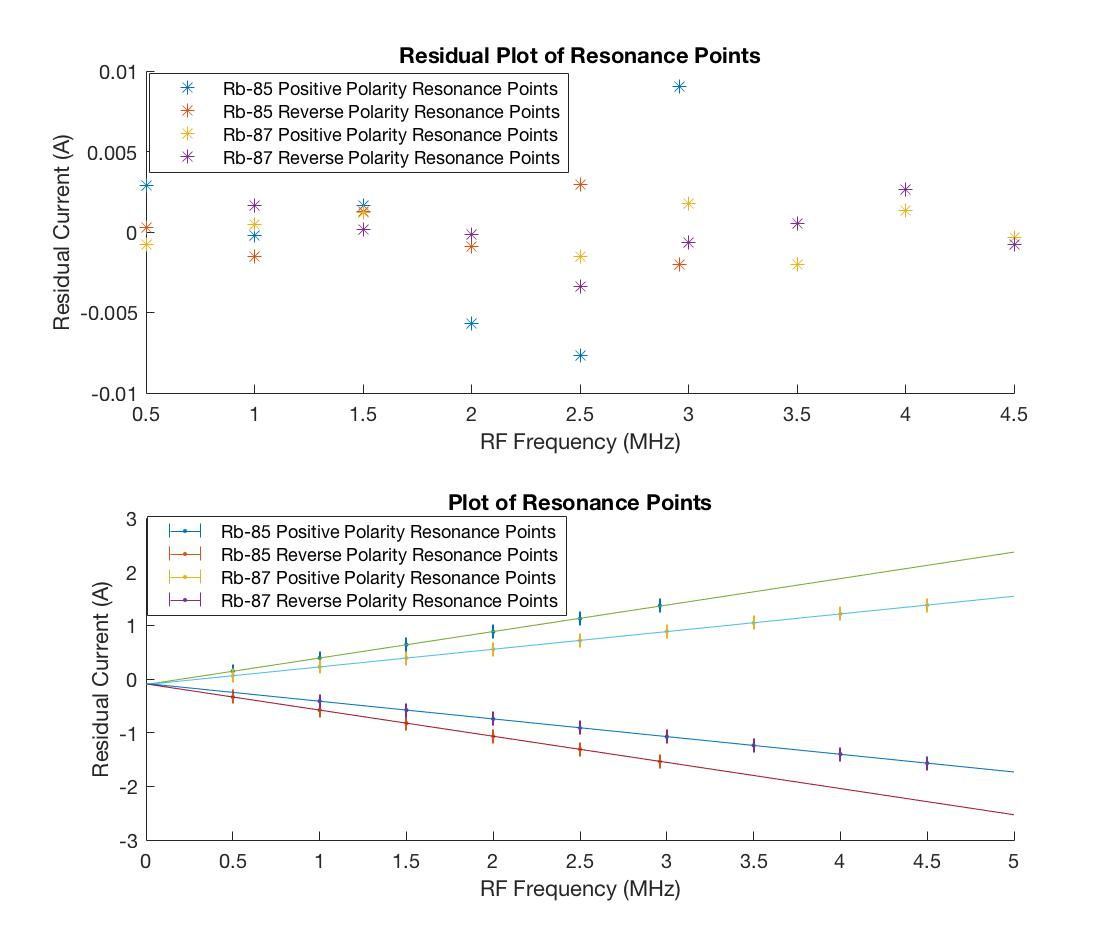
\includegraphics[scale = 0.25]{2.jpg}
        \caption{Plot of Resonance Points Described Through Functional Inverse i(f), with Best Fit Lines}
        \label{fig:my_label}
    \end{figure}
\indent We calculate the reduced Chi-Squared value through:
\begin{equation}
        \tilde{\chi}^2 = \frac{\sum_i (i_i - i(f_i))}{\Delta i^2*d} = \frac{\sum_i (i_i - (m'*f_i + b'))}{\Delta i^2*d}
\end{equation}
where $i_i$ and $f_i$ are the observed resonant current and frequencies and d = N-2 is the degrees of freedom for N data points (d = N-2 because two fit parameters were calculated). 
\\\indent We calculated the $R^2$ coefficient of determination by utilizing the following expression \cite{rsq}:
\begin{equation}
        R^2 = 1- \frac{\sum_{i=1}^N (i_i - i(f_i))^2}{\sum_{i=1}^N (i_i - \frac{1}{N}*\sum_{j=1}^N i_j)^2}
\end{equation}   
Plugging in our $\Delta i$ from each data set (isotope and polarity of current), N (number of data points in set), and all $f_i$ and $i_i$ data points, and we attain the following $\tilde{\chi}^2$ and $R^2$ values:
\begin{table}[H]
\centering
\caption{$\tilde{\chi}^2$ and $R^2$ for Best Fit Lines}
\label{my-label}
\scalebox{0.7}{
\begin{tabular}{llll}
\textbf{Isotope} & \textbf{Current Polarity} & \textbf{$\tilde{\chi}^2$} & \textbf{$R^2$} \\
85Rb & Positive & 3.921 & 0.9998 \\
85Rb & Negative & 0.2421 & 1.000 \\
87Rb & Positive & 0.0778 & 1.000 \\
87Rb & Negative & 0.2661 & 1.000
\end{tabular}}
\end{table}
Judging by the $R^2$ values, we see that the model very accurately predicts the data. In the cases of 85Rb-Positive, 85Rb-Negative 87Rb-Negative, their reduced chi-squared values (on the order of one) indicate a nicely fitting model ($\tilde{\chi}^2 \sim 1$). However, for the other two models, we see that the found $\Delta i$ values were a bit too large as compared to the residuals of the data, meaning that many different models could describe our data. Nevertheless, we have attained relatively predictive models of resonance RF frequency as a function of current. Later on in the analysis we will be modifying $\Delta i$ due to an assumption about the Breit-Rabi equation in the case we assume that the equation is a perfect description for our model. However, the point is not relevant to our next immediate analysis.
\\\indent To find the nuclear spins $I_1$ and $I_2$ of 85-Rb and 87-Rb respectively, we employ a few different methods. According to the Breit-Rabi equation (for positive polarity current + and reverse polarity current -, we use this model because we reasonably predictive linear fit models) eq.(13):
\begin{equation}
        f_\pm(i) = \frac{2.799}{2I+1}*(\frac{\lambda*Ni}{A} \pm B_E)
\end{equation}
where N is the number of turns in the Helmholtz coils (found to be 135 turns) and A, the radius of the coils, was found to be 0.275 m (no error bounds given). For now, we make the assumption that the 2.799 and $\lambda$ constants are at their correct values (partially in line with our assumption about a uniform externally applied magnetic field). Using two of the four models that are either both positive polarity or both negative polarity, we divide the slopes of the two best-fit lines of isotopes Rb-87 (slope $m_2$) and Rb-85 (slope $m_1$) to find:
\begin{equation}
        \frac{m_2}{m_1} = \frac{2*I_1 + 1}{2*I_2 + 1} = \frac{k_1}{k_2}
\end{equation}
Using $m_1$ and $m_2$ from the positive and reverse polarity cases, we find $\frac{m_2}{m_1}$: $\frac{m_2}{m_1}_+ = 1.4995$, and $\frac{m_2}{m_1}_- = 1.4791$.
With the assumption that nuclear spins of the isotopes take on half-integral values (2I + 1 = k = 1,2,...), error analysis here is unwarranted, but also we can use this fact to find possible values for $I_1$ and $I_2$. We see that such $\frac{m_2}{m_1}$ value is approximately $\frac{3}{2}$. From this relationship, we can yield the following pairs of spins. The lowest $k_1$ can be is 3 and the lowest $k_2$ can be is 2. For such values, the pair of spins ($I_1,I_2$) is ($1,\frac{1}{2}$). To hold the relationship $\frac{k_1}{k_2} = \frac{3}{2}$ next $k_1, k_2$ values are 6 and 4 respectively, yielding ($I_1,I_2$) = ($\frac{5}{2},\frac{3}{2}$). And so we can see that the possible values for nuclear spins ($I_1,I_2$) = (1+$\frac{3n}{2}$,$\frac{1}{2}+n$) for n = 0,1,2,3,...$\infty$, according to the relationship derived above. This is a particularly poor and non illuminating way of finding the nuclear spins of the isotopes of rubidium, as we cannot pinpoint the exact spin combination. There are far more effective ways to find the spin values (for instance, conducting spectroscopy on the Zeeman splittings of the hyperfine levels of rubidium to find the original degeneracy and thus F-value of the hyperfine system).
\\\indent Now we will make a grand assumption by which to complete the rest of our calculations. We will assume that the quantum mechanics used to derive the Breit-Rabi law in the low field case holds true, and thus the equation describing this law is also the perfect equation to describe our four isotope/polarity linear models f = m*i + b. Thus, we must come up with an error for each datapoint $\Delta i$ such that the Breit-Rabi law is the perfect model for our data. Under our assumption, such a $\Delta i$ can account for any sources of systematic and random error, and any other reasons why our previous model was not the best fit. Such a model has $\tilde{\chi}^2$ = 1. So we can estimate a new $\Delta i$ for each model such that $\tilde{\chi}_{new}^2$ = 1. We see:
\begin{equation}
      \frac{\Delta i_{new}^2}{\Delta i_{old}^2} = \frac{\tilde{\chi}_{old}^2}{\tilde{\chi}_{new}^2}, \Delta i_{new} = \Delta i_{old} * \sqrt{\tilde{\chi}_{old}^2}
\end{equation}
Plugging in $\Delta i_{old}$ and $\sqrt{\tilde{\chi}_{old}^2}$ found from the previous four models, and we find $\Delta i_{new}$ = 0.0068 A, 0.0021 A, 0.0014 A, 0.0019 A (not to confuse amps with the radius A of the Breit-Rabi law) for 85Rb-Positive, 85Rb-Reverse, 85Rb-Positive, 87Rb-Reverse cases respectively. We may use this data in future data analyses. Returning to the model, f = m*i + b, we can also find the spins from the slope m via the Breit-Rabi Law ($m = \frac{2.799*\lambda * N}{(2I+1)A}$). Rearranging this, we find that:
\begin{equation}
      I \approx \frac{2.799 \lambda N}{2*|m|*A} - \frac{1}{2}
\end{equation}
with associated error
\begin{equation}
      \sigma_I = \sigma_m * |\frac{dI}{dm}| = \frac{\sigma_m*I}{|m|}
\end{equation}
Plugging in the m and $\sigma_m$ values found previously, N = 135, using 2.799 MHz/gauss, $\lambda = 0.9 * 10^{-6} \frac{tesla*meter}{amps}$, and A = 0.275m, and we find that for positive polarity, $I_1 = 2.5514\pm0.0170$ and $I_2 = 1.5350\pm0.0014$, and for negative/reverse polarity, $I_1 = 2.5143\pm0.0167$ and $I_2 = 1.5380\pm0.0024$. Of course, here we can still use the assumption that I is half integral. We find the pair of possible nuclear spin values, ($I_1,I_2$) = (1+$\frac{3n}{2}$,$\frac{1}{2}+n$) for n = 0,1,2,3,...$\infty$ by finding the n value where the nuclear spins and their errors are closest to a pair of spins described by an n value. We see that ($I_1,I_2$) = ($\frac{5}{2},\frac{3}{2}$) (only in the 85Rb- case does the true spin lie within this interval). Again, a proper error analysis is unnecessary because of the assumption we made about nuclear spins being half integral, but the two analyses on spins show some agreement. %fix spin and spin error, and ADD values from the top!!!! near pm
% mention spectroscopy and how this is a bad way of doing it... multiple spin values you can find... We make the Breit Rabi law by changing delta i to estimate spins and see if that particular spin lies within spin interval
\\\indent We still hold that our assumption about Breit-Rabi's law being the perfect model. We will use this to find the value of the Earth's magnetic field (or some field that is a result of the interference between Earth's magnetic field and other confounding fields). For each of the four linear models, we set current i equal to zero to find the intercept. Because we assumed the Breit-Rabi's law is the perfect model to describe our linear fits ($\tilde{\chi}^2$=1), we also set the current equal to zero and equate the intercepts between the lines of best fit and the Breit-Rabi law, and if we rearrange this:
\begin{equation}
      b_\pm = \frac{\pm2.799*B_E}{2*I + 1} \rightarrow B_{E_\pm} = \pm\frac{b*(2*I + 1)}{2.799}
\end{equation}
with error:
\begin{equation}
      \sigma_{B_E} = \frac{\sigma_b*(2*I + 1)}{2.799}
\end{equation}
For $\pm$ current polarity cases. Nuclear spin, I, has no associated error (no error propagation) because of the aforementioned assumptions. Plugging in values of I [($I_1,I_2$) = ($\frac{5}{2},\frac{3}{2}$)], b, $\sigma_b$, and using the correct units for the 2.799 constant, we find Earth's magnetic field to be (for cases Rb: $85+,85-,87+, 87-$):
\begin{equation}
      \begin{array}{c}
           B_{E_{85+}} = 0.4462 \pm 0.0250 gauss\\
           B_{E_{85-}} = 0.4032 \pm 0.0300 gauss\\
           B_{E_{87+}} = 0.4502 \pm 0.0040 gauss\\
           B_{E_{87-}} = 0.3670 \pm 0.0083 gauss
      \end{array}
\end{equation}
The earth's magnetic field is plotted below with its associated errors:
\begin{figure}[H] %FIX
        \centering
        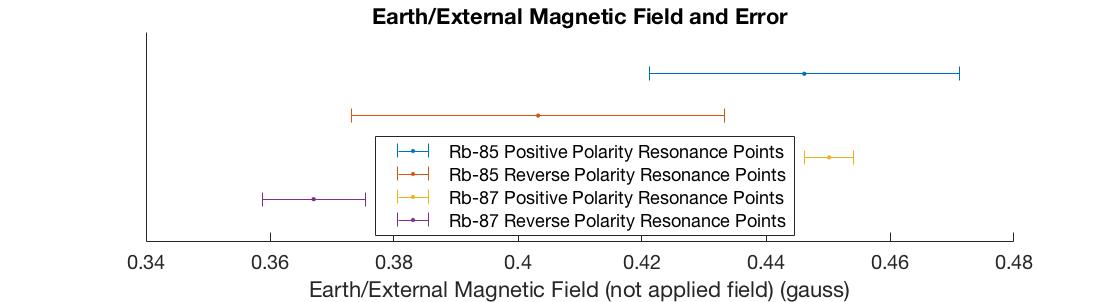
\includegraphics[scale = 0.25]{3.jpg}
        \caption{Found Earth Magnetic Field with Errors}
        \label{fig:my_label}
    \end{figure}
\indent In this case, we do not truly have an accepted value for Earth's magnetic field (globally Earth's field is inhomogenous). However, research indicates that Earth's surface magnetic field ranges from 0.25 gauss to 0.65 gauss. \cite{earth}
Furthermore, we accept that there are many sources of interference that could have impacted our field measurements and affected the findings of our resonance points (to be discussed in conclusion). The fields we have found are well in the order of the postulated field values and according to the figure above, the fields generally agree with each other due to their overlapping uncertainty intervals. % Explain importance of agreement
The field values we found from the intercept certainly could have been influenced from Earth's magnetic field, and are of the order of magnitude.
\\\indent Regarding the temperature dependence of the signal strength coming from the rubidium sample, we found an 85Rb- (85-Rubidium negative polarity) resonance point as specified in the table 5. We plotted the temperature versus max voltage (found via the method described in the procedure) below. 
\begin{figure}[H] %FIX
        \centering
        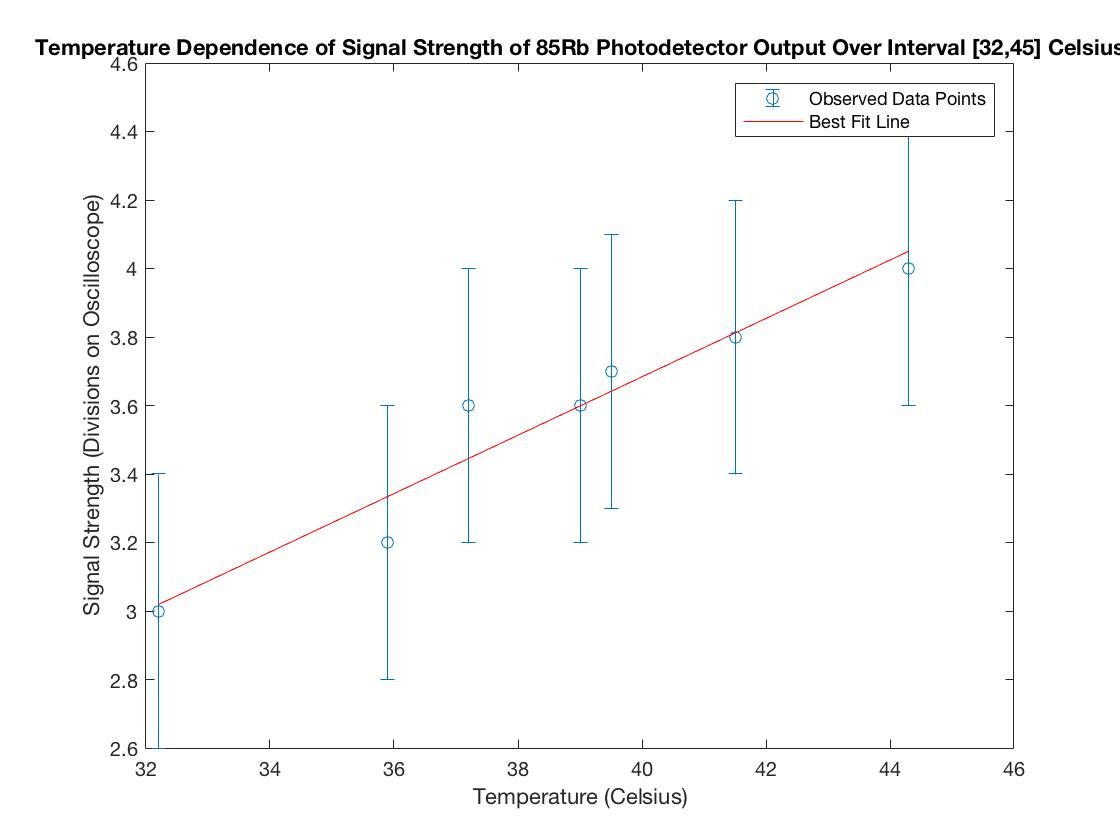
\includegraphics[scale = 0.25]{4.jpg}
        \caption{Temperature Dependence of Signal Strength}
        \label{fig:my_label}
    \end{figure}
\indent The data is plotted in units of oscilloscope output divisions, and the conversion to voltage is given in the table. However, it is not to do this necessary for this analysis. We did not measure over the entire temperature range of the bulb. However, we did measure a large enough range to notice a general trend. Performing a linear fit on the data using aforementioned methods, we found the best fit line of temperature (T) versus signal (V) to be:
\begin{equation}
      V(T) \approx 0.085*T + 0.27  divisions
\end{equation}
with a corresponding calculated (using matlab) $R^2$ value of 0.94. This is a reasonable predictive model, though the large error values due to the fuzziness of the picture we were seeing could have driven down goodness of fit measures such as chi-squared. We do note that this is a relatively strong trend, but only for a limited temperature range. We should not extrapolate this linear model because of the relatively nonlinear and confounding effects (eg. reduction in the lifetime of optically pumped states due to increasing vapor density) that can cause the signal to decrease at even higher temperatures and increase at a lower range. Such a line does demonstrate some temperature dependence of the signal strength.
\\\indent After turning off the RF generator (f = 0), we varied the current while looking for resonance in order to find the Zero Field Resonance. With a 40$\degree C$ sample temperature and temperature control off, we found the resonance point to be at a current value of -0.0936 Amps. We will come back to discuss this result in the conclusion.
\\\indent With the experimental setup in proper conditions for measuring pumping and relaxation times for a resonance point of 85Rb (resonance point found to be (i = -1.0056 amps,f = 1.85 MHz); also playing around with preamp settings), the more abundant isotope inside the sample, we took a high speed video of the optical pumping and relaxation effects over one cycle of square modulation. On the scope, we used settings of channel 1 (square modulation wave) at 1 volt per division and 2 (output from photodetector) at 0.1 volts per division and the horizontal divisions were each 0.5 seconds. In the raw data, you can find sampled video images detailing what we were seeing on the oscilloscope during pumping/relaxation. Using MATLAB, we ran a video stabilization algorithm that stabilized and fix the video with very limited wobble about the scope axes. After doing that, we were able to find data points of the channel 2 signal (V) over time elapsed (t). We did by displaying one out of every five frames (over the pumping and relaxation intervals) to the user and allowing them to graphically input the position of the pumped/relaxed signal (t,V) for each of these frames (we assumed that any measurement errors introduced here are the same and thus not neccessary in error analysis). We also allowed the user to graphically determine the start data point of the pumping, start data point of the relaxation and end data point of the relaxation. The data was divided into two sets, one for the (t,V) points for pumping and another for relaxation. Three points were chosen for calibration, $\vec{x_1},\vec{x_2},$ and $\vec{x_3}$. $\vec{x_1}$ is the vector that is from the origin of the image to a particular point chosen by which the rest of the data points will be found relative to it; the point lies in the intersection between two lines in the scope's display grid. $\vec{x_2}$ was defined to be three horizontal scope divisions to the right of $\vec{x_1}$, and $\vec{x_3}$ was defined to be three vertical scope divisions below $\vec{x_1}$. Relative vectors $\vec{r_t} = \vec{x_2}-\vec{x_1}$ and $\vec{r_V} = \vec{x_3}-\vec{x_1}$ were calculated, as well as distances ($d_t = |\vec{r_t}|$ and $d_V = |\vec{r_V}|$) and unit vectors that point along the scope's horizontal and vertical lines ($\hat{r_t} = \frac{\vec{r_t}}{|\vec{r_t}|}$ and $\hat{r_V} = \frac{\vec{r_V}}{|\vec{r_V}|}$, respectively). A conversion factor between pixels and volts/time was established by the fact that the number of pixels that describe $d_t$ are equivalent to 3*0.5 seconds = 1.5 seconds and likewise $d_V$ is equivalent to 0.3 Volts. Thus, we convert between volts/seconds and pixels along axes described by $\hat{r_V}$ and $\hat{r_t}$ respectively through conversion factors $\gamma_V = \frac{0.3 volts}{d_V}$ and $\gamma_t = \frac{1.5 seconds}{d_t}$ where the two d values are in pixels. The set of all measured $\{\vec{x_p}\}$ vectors describe pumping data points (t,V) and the set $\{\vec{x_R}\}$ vectors describe relaxation data points. However, the (t,V) points aforementioned are not the actual (t,V) points being measured on the oscilloscope because the data points are being measured in the Cartesian plane, which does not account for the actual directions in which we measure the data (we wish to measure data points along Span$\{\hat{r_t},\hat{r_V}\}$).
\begin{figure}[H] %FIX
        \centering
        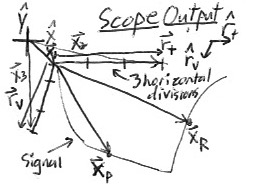
\includegraphics[scale = 0.4]{12.jpg}
        \caption{Visual Description of Vector Analysis of Scope Output for Pumping/ Relaxation Times}
        \label{fig:my_label}
    \end{figure}
In order to best measure our (t,V) data points in their proper units and coordinate system, we convert the $\{\vec{x_p}\}$ and $\{\vec{x_R}\}$ points to Span$\{\hat{r_t},\hat{r_V}\}$ coordinates through the following conversion (suppose $\vec{x_p}$ and $\vec{x_R}$ each represent a data point):
\begin{equation}
      [\vec{r_{p/R}}] = ((\vec{x_{p/R}}-\vec{x_1})\cdot\hat{r_t}*\gamma_t,(\vec{x_{p/R}}-\vec{x_1})\cdot\hat{r_V}*\gamma_V) = (t,V)
\end{equation}
and now we have the actual signal V and time elapsed t measurements relative to $\vec{x_1}$, measured using the coordinate system mapped out by plane Span$\{\hat{r_t},\hat{r_V}\}$. Note how the data points are flipped from the points displayed on the scope. We plot these points below, separating the two data sets:
\begin{figure}[H] %FIX
        \centering
        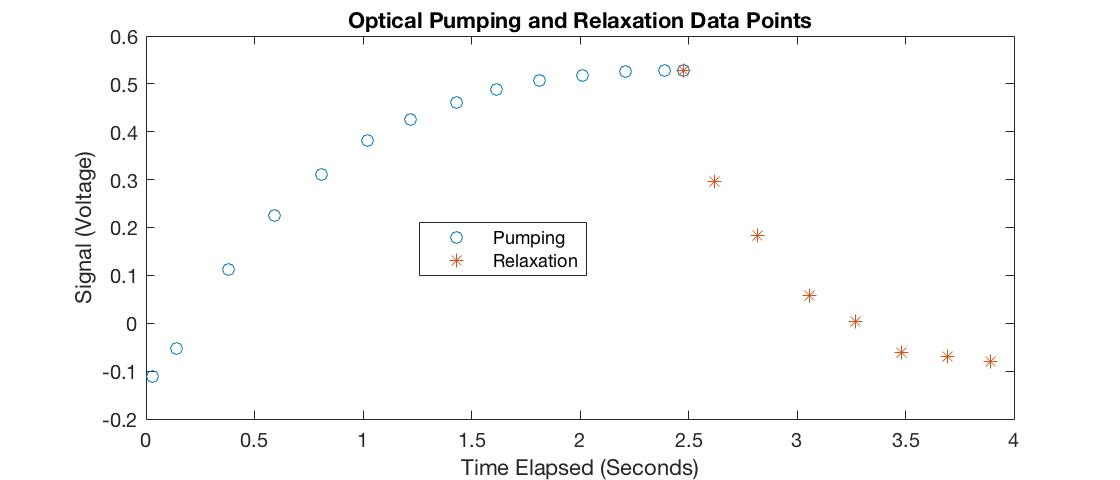
\includegraphics[scale = 0.25]{5.jpg}
        \caption{Pumping and Relaxation Data Points For Square Wave Modulation of RF Signal}
        \label{fig:my_label}
    \end{figure}
We translated all of these $\{[\vec{r_{p/R}}]\}$ data points by subtracting out the minimum t and V points for both the pumping and relaxation points separately. After the applied transformation to the data, the pumping curve can be modelled by the function $V_p(t) = a*(1-e^{\frac{-t}{\tau_p}})$, and the relaxation curve can be modelled by the function $V_R(t) = a*e^{\frac{-t}{\tau_R}}$, where $\tau_p$ and $\tau_R$ are the approximate pumping and relaxation times, or the time it takes for the signal to change by $a*\frac{1}{e}$ (i.e. setting $V_p(t) = a*(1-\frac{1}{e})$ and $V_R(t) = a*\frac{1}{e}$). We fit data points of $(t,V_p(t))$ and $(t,V_R(t))$ (t is the elapsed time since the start of either pumping or relaxation) to each of the corresponding models through the use of least-squares regression. We found that $\tau_p \approx 0.819$ seconds with a $95\%$ confidence interval of [0.742, 0.897] seconds and $\tau_R \approx 0.374$ seconds with a $95\%$ confidence interval of [0.315, 0.433] seconds. We calculated correlational adjusted $R^2$ values that would indicate how well the data points fit the model.
\begin{equation}
      R_{adj}^2 = 1-\frac{(1-R^2)(n-1)}{n-k-1}
\end{equation}
where $R^2$ has been calculated using eq.(22) by substituting i for V and f for t, n is the number of data points included (14 for pumping and 8 for relaxation), and k is the number of fit parameters (2 for each model) \cite{stats}. We find that the adjusted $R^2$ value for pumping is 0.9965 and for relaxation this is 0.9900, both indicating highly predictive models. The pumping and relaxation data points with their best fit curves have been plotted below:
\begin{figure}[H] %FIX
        \centering
        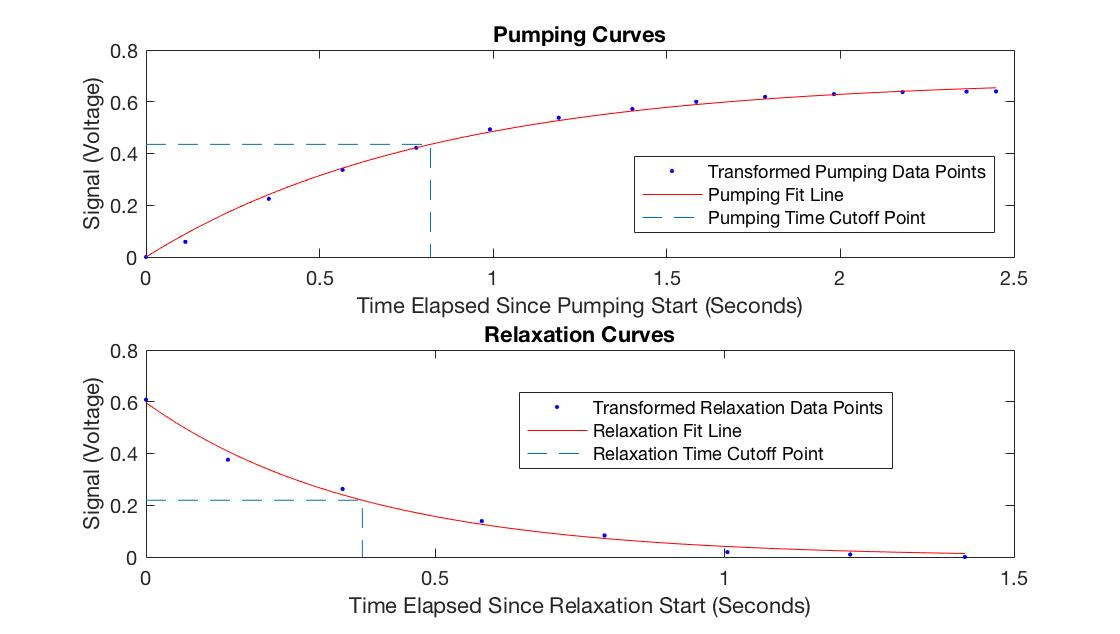
\includegraphics[scale = 0.25]{6.jpg}
        \caption{Pumping and Relaxation Transformed Data With Best Fit Exponential Curves}
        \label{fig:my_label}
    \end{figure}


%flip
%$\{\vec{r_p}\}$ for pum


% agreement between 4 x-intercepts of Be
% add error bars
% measured at different times
% time it takes to switch polarity
% etc

\section{Conclusion}
    %start conclusion here
    \subsection{Results and Discussion of Results}
    The discretized energy levels from which we can observe a quantum system can tell us a lot about it. In this experiment, we studied the energy levels that result from coulomb interaction, fine, hyperfine, and zeeman splitting effects. We were able to measure the magnitude of some of these Zeeman energy spacings through the use of optical pumping, in which we excited a distribution of quantum states into higher energy states using circularly polarized light (selection rules of simulated emission, absorption, and spontaneous emission favoring higher energies). By introducing an RF transition that was the same energy as the Zeeman splitting, we were able to relax the energy states into the original distribution. Oscillating the size of the Zeeman splittings about the RF transition through the modulation of the magnetic field enabled us to find points of resonance. To do all of this, we used an apparatus that heated up a gas sample of two isotopes of Rubidium, shined circularly polarized light on the sample, applied a modulating external magnetic field and RF frequency light to the sample. We were able to conduct measurements by converting the resulting light passing through the sample at the end of a photodetector and measuring it using an oscilloscope.
    \\\indent Our main two goals in this experiment were to find the nuclear spins of $^{85}Rb$ and $^{87}Rb$ and measuring Earth's magnetic field. We did this by fitting lines to the points of resonance that we found, and comparing the parameters describing this line to the Breit-Rabi equation with the equation for a helmholtz magnetic field substituted into it. We did this for both isotopes of rubidium and for the cases in which the current running through the helmholtz coils had positive and reverse/negative polarity, producing four separate lines.
    \\\indent Under the assumption that the Breit-Rabi law is a great model for our data (which our reduce chi-square values and $R^2$ values indicated that they were decent to good fitting lines), we calculated the spins of $^{85}Rb$ ($I_1$) and $^{87}Rb$ ($I_2$), which were found in the positive polarity case to be $I_1 = 2.5514\pm0.0170$ and $I_2 = 1.5350\pm0.0014$, and for reverse polarity, $I_1 = 2.5143\pm0.0167$ and $I_2 = 1.5380\pm0.0024$. Also, finding the ratio of $\frac{2*I_1+1}{2*I_2 + 1}$ for the positive polarity case (1.4995), and for the negative polarity case (1.4791), and under the assumption that in quantum mechanics, spin can only take on half integral values, we ultimately found the spins to equal: $I_1 = \frac{5}{2}$ and $I_2 = \frac{3}{2}$, which conforms to our expectations. This, however, is not an ideal method of finding the nuclear spins of rubidium isotopes, as the aforementioned ratio of spins and an assumption that spin is half integral could not help us deduce which half integer values were our correct spin values. Using spectroscopy that would enable us to directly see the energy level splittings may serve as a better way to deduce the spin values. From the atomic physics lab, we can utilize a Fabry-Perot interferometer or monochromator to directly see the Zeeman or hyperfine splittings of rubidium (assuming the design provides high enough resolution), and the number of split lines found after a magnetic field is applied should allow us to deduce the degeneracy of the states before splitting. Through some derivation, we could use this information to calculate the spins of Rubidium. 
    \\\indent We used similar assumptions (perfect model and half integral spin) to deduce the value of the earth's magnetic field. Performing a similar manipulation of the Breit-Rabi law in accordance with the four found lines of best fit, we were able to find earth's magnetic field for the 85Rb and 87Rb lines in the positive polarity case to be 0.4462 $\pm$ 0.0250 gauss and 0.4502 $\pm$ 0.0040 gauss respectively, and in the reverse polarity case to be 0.4032 $\pm$ 0.0300 gauss and 0.3670 $\pm$ 0.0083 gauss respectively. For the validity and precision of the experiment data, it is important that the found fields all overlapped with each other from their error intervals. However, this $Rb85_-$'s earth's magnetic field measurement was able to overlap with two other fields, but each of the other found fields only overlapped with one of the other magnetic field error intervals. Though the order of magnitude of the found fields were the same as an interval of field values describing earth's field, we can suggest that it was not just earth's field that we were measuring. We know that earth's magnetic field varies at the surface, but due to the localization of our experimental setup, and how the field should not vary by too much over time, we can conclude that many other interfering magnetic fields confounded our data. Perhaps, as well, the Briet-Rabi law and the assumptions set forth by our derivation of the helmholtz field (constant field at the center), are not as valid as we would like to think.This will be discussed in the next subsection.
    \\\indent We noticed a linearly positive trend in the signal strength as a function of the temperature of the sample. The temperature interval taken over was a subset of the the total temperature range, but the data was convincing enough to establish a correlational inference as to that the signal strength for 85Rb depends on the temperature of the sample, with some of the effects described in the theory level. One draw back is that the data here cannot be extrapolated to the 87Rb case and for other temperature or resonance points values.
    \\\indent We found the Zero Field resonance point of the sample to be at an i value of -0.0936 amps. 
    \begin{figure}[H] %FIX
        \centering
        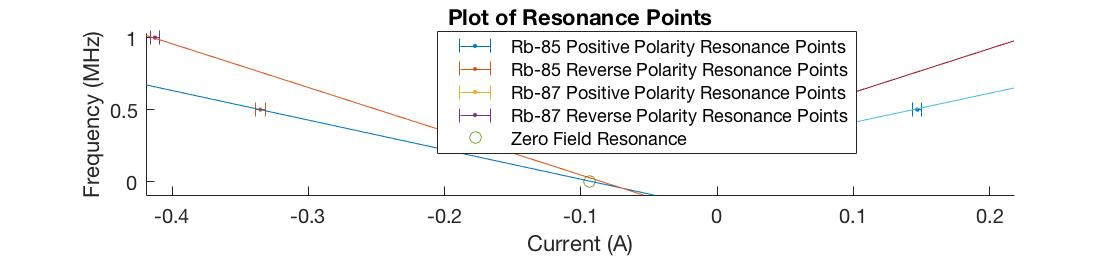
\includegraphics[scale = 0.25]{7.jpg}
        \caption{Zoomed in Plot of Resonance Points Revealing a Zero Field Resonance Point}
        \label{fig:my_label}
    \end{figure}
    Returning to our plot of resonance points, we see that this point lies on the line of Rb85 Reverse Polarity (it was measured with negative polarity and with the 85Rb part of the sample). What is interesting is that at this point, the externally applied field and the earth's magnetic field (and other interfering fields), cancel out, and we are left with zero Zeeman splittings with an RF transition at 0 J. How is it that we are able to still see transitions? With no applied RF frequency light, the net magnetic field is seemingly zero, and the Zeeman splittings, are in fact, very close to zero. Nonetheless, we could not make them exactly zero, especially due to background noise (eg. light, time varying magnetic fields from surrounding circuitry). These sources of background interference can cause optical pumping and a quick relaxation from energy states very close to one another (these sources essentially introduce RF transitions). Spontaneous emission is also much more possible as the small energy spacings of the zeeman splittings approach the order of magnitude of the nonzero energy widths due to the quantum mechanical uncertainty between energy and the lifetime of a particular quantum state. With an RF frequency of 0, yielding light of infinitely large wavelength (constant voltage offset), we can still have spontaneous transitions between the near degenerate energy states.
    \\\indent We were able to estimate the optical pumping and relaxation times of 85 Rb ($\tau_p$ and $\tau_R$ respectively) after applying square wave modulation to the RF light. We estimated $\tau_p \approx 0.819$ seconds and $\tau_R \approx 0.374$ seconds with 95$\%$ confidence intervals of [0.742, 0.897] and [0.315, 0.433] seconds respectively using a relatively predictive model.
    
    
    \subsection{Some Possible Sources of Error}
    % inhomogeneous field, other interfering fields, time it takes to switch polarity, noise in the preamp, interfering light, temperature of coils changing over time, 
    There are a number of sources of error that could have interfered in measuring the spin and earth's magnetic field. Most notably, there are many interfering fields that introduce time dependent perturbations to our energy levels. These could come from nearby compasses, the electronics in our phones, wires around the laboratories, fields generated by moving the our rolling chairs, and there are many other sources. We also assume that our applied field in our experimental set up is either parallel or anti-parallel to earth's magnetic field. However, this may not be true, and along with the fact that the helmholtz coils do not produce a truly constant and homogenous field at the location of the gas sample, we see that there may be some misalignment between the magnetic dipole formed by the quantum system and the external magnetic field, which can cause energy transitions that do not correspond to the transitions experienced during optical pumping.
    \\\indent In finding our resonance points, there were a lot of bumps in the lemniscate figure that made it quite difficult to discern if we had found a point of resonance. Regardless of the noise, this is because of phase differences introduced by the signal of the modulating magnetic field. Some of the phase differences were introduced during different boundary reflections as the signal was transmitted to different devices, others were introduced by induced capacitance and inductance in the BNC cables as they were twisted and turned. In retrospect, a terminator could have reduced some of these internal reflections. Such bumps introduced additional measurement and systematic error into our analysis.
    \\\indent Depending on the temperature of the sample, additional thermal broadening effects may have changed the definite energy levels and energy distribution of particles. For the zero field resonance, additional errors were introduced through interference effects from nearby light sources prompting stimulated emission from the pumped state to a relaxed state. Regarding our discovery of the pumping and relaxation times, there is still some wobble in the camera as we record, only a subset of the total number of data points were chosen, and the graphical input of the user could have been error prone if the user did not select the exact point of the center of the pumping signal. These present other sources of error in our experiment. As with all experiments, these are some of the sources of error, and future experiments would have to reduce these sources.
    
    \subsection{Final Thoughts}
    The Optical Pumping experiment was a very quick and easy way for me to explore some of the foundations of quantum mechanics. I really enjoyed learning more about energy splittings and deriving the Breit-Rabi law. However, from this experiment, I see that there are limitations in applying my knowledge of quantum mechanics into experimental design. I really liked the design of the experiment, but I do agree that maybe some spectroscopy could help aid our conclusions. That being said, every experiment has limitations, and one key limitation here is how much interference from the outside and how much noise is one willing to withstand as they go about experimenting. Again, great lab, and thank you for giving me the opportunity to solidify my understanding about this subject matter.

\section{Acknowledgments}

I would like to thank my lab partner and Matlab programming.

\section{References}

\begin{thebibliography}{1} %change this

  \bibitem{opt} "Optical Pumping Lab" Don Orlando Berkeley, 2016. Web Address: http://experimentationlab.berkeley.edu/OPT#Data$\_$Analysis 

  \bibitem{err}  "Introduction to Error Analysis". John R. Taylor, University of Colorado, 1997. University Science Books.

  \bibitem{nuc} "Nuclear Moments". N. Ramsey, 1953. UC Berkeley Physics Library Reprints.
  
  \bibitem{function} "MODEL DS345 Synthesized Function Generator". Stanford Research Systems. 2009. Web Address: http://physics111.lib.berkeley.edu/Physics111/Equipment$\_$Manuals/SRS/DS345m.pdf
  
  \bibitem{rsq} "Coefficient of Determination". Wikipedia. 2017. Web Address: "https://en.wikipedia.org/wiki/Coefficient$\_$of$\_$determination"
  
  \bibitem{earth} "Earth's Magnetic Field". Wikipedia. 2017. Web Address: "https://en.wikipedia.org/wiki/Earth$\%$27s$\_$magnetic$\_$field "

  \bibitem{stats} "Adjusted R2 / Adjusted R-Squared: What is it used for?". Statistics How To. 2017. Web Address: "http://www.statisticshowto.com/adjusted-r2/"
  
  \bibitem{fs} "Fine Structure of Hydrogen". Richard Fitzpatrick, 2010. Web Address: "http://farside.ph.utexas.edu/teaching/qmech/". 

  \end{thebibliography}

\section{Raw Data}
%HOW TO IMPORT THE VIDEO?? IMAGES???
\begin{table}[H]
  \centering
  \caption{Resonance Points}
  \scalebox{0.6}{
    \begin{tabular}{rrr|rrr}
    \multicolumn{1}{l}{\textbf{Isotope:}} & \multicolumn{1}{l}{\textbf{Polarity: }} & \multicolumn{1}{l|}{\textbf{Polarity: }} & \multicolumn{1}{l}{\textbf{Isotope:}} & \multicolumn{1}{l}{\textbf{Polarity: }} & \multicolumn{1}{l}{\textbf{Polarity: }} \\
    \multicolumn{1}{l}{ $^{85}Rb$} & \multicolumn{1}{l}{Positive} & \multicolumn{1}{l|}{Reverse} & \multicolumn{1}{l}{ $^{87}Rb$} & \multicolumn{1}{l}{Positive} & \multicolumn{1}{l}{Reverse} \\
    \multicolumn{1}{l}{\textbf{Modulation Amplitude:}} & 50    & 50    & \multicolumn{1}{l}{\textbf{Modulation Amplitude:}} & 40    & 40 \\
    \multicolumn{1}{l}{\textbf{Temperature $\degree$C:}} & 40    & 42.5  & \multicolumn{1}{l}{\textbf{Temperature $\degree$C:}} & 42.5  & 42.6 \\
    \multicolumn{1}{l}{\textbf{Frequency (MHz)}} & \multicolumn{1}{l}{\textbf{Current (A)}} & \multicolumn{1}{l|}{\textbf{Current (A)}} & \multicolumn{1}{l}{\textbf{Frequency (MHz)}} & \multicolumn{1}{l}{\textbf{Current (A)}} & \multicolumn{1}{l}{\textbf{Current (A)}} \\
    2.96  & 1.3670 & -1.5367 & 4.5   & 1.3770 & -1.5686 \\
    2.5   & 1.1233 & -1.3075 & 4     & 1.2141 & -1.4004 \\
    2     & 0.8786 & -1.0676 & 3.5   & 1.0462 & -1.2377 \\
    1.5   & 0.6392 & -0.8217 & 3     & 0.8854 & -1.0741 \\
    1     & 0.3906 & -0.5807 & 2.5   & 0.7176 & -0.912 \\
    0.5   & 0.1470 & -0.3352 & 2     & 0.5544 & -0.7440 \\
          &       &       & 1.5   & 0.3912 & -0.5789 \\
          &       &       & 1     & 0.2259 & -0.4126 \\
          &       &       & 0.5   & 0.0601 &  \\
    \end{tabular}}%
  \label{tab:addlabel}%
\end{table}%

\begin{table}[H]
  \centering
  \caption{Current Values for $\Delta i$ Calculation}
  \scalebox{0.6}{
    \begin{tabular}{rrrrr}
    \multicolumn{1}{l}{\textbf{Isotope:}} & \multicolumn{1}{l}{85-Rb} & \multicolumn{1}{l}{85-Rb} & \multicolumn{1}{l}{87-Rb} & \multicolumn{1}{l}{87-Rb} \\
    \multicolumn{1}{l}{\textbf{Polarity:}} & \multicolumn{1}{l}{Positive} & \multicolumn{1}{l}{Reverse} & \multicolumn{1}{l}{Positive} & \multicolumn{1}{l}{Reverse} \\
    \multicolumn{1}{l}{\textbf{Resonance Frequency (MHz):}} & 2.96  & 2.96  & 4.5   & 4.5 \\
    \multicolumn{1}{l}{\textbf{Modulation Amplitude}} & \multicolumn{1}{l}{\textbf{Current Values (A)}} & \multicolumn{1}{l}{\textbf{Current Values (A)}} & \multicolumn{1}{l}{\textbf{Current Values (A)}} & \multicolumn{1}{l}{\textbf{Current Values (A)}} \\
    10    & 1.3692 & -1.5350 & 1.3765 & -1.5647 \\
    20    & 1.3603 & -1.5444 & 1.3858 & -1.5736 \\
    30    & 1.3676 & -1.5413 & 1.3855 & -1.5735 \\
    40    & 1.3670 & -1.5439 & 1.3770 & -1.5686 \\
    50    & 1.3669 & -1.5367 & 1.3862 & -1.5710 \\
       
    \end{tabular}}%
  \label{tab:addlabel}%
  \end{table}


\begin{table}[H]
\centering
\caption{Temperature versus Observed Max Signal Data Points ofr Rb 85}
\label{my-label}
\scalebox{0.6}{
\begin{tabular}{lll}
\multicolumn{1}{l|}{\textbf{Resonance Point:}} & \textbf{B-field Modulation Amplitude=} & \textbf{50} \\ \hline
\multicolumn{1}{l|}{\textbf{Current = -1.0115 Amps}} & \multicolumn{1}{l|}{\textbf{Volts/Div = 50 mV/div}} & \textbf{Frequency = 1.85 MHz} \\ \hline
\textbf{Temperature ($\degree$C)} & \textbf{Max Voltage (divs)} & \textbf{$\sigma_V$(divs)} \\
32.2 & 3 & 0.4 \\
35.9 & 3.2 & 0.4 \\
37.2 & 3.6 & 0.4 \\
39 & 3.6 & 0.4 \\
39.5 & 3.7 & 0.4 \\
41.5 & 3.8 & 0.4 \\
44.3 & 4 & 0.4
\end{tabular}}
\end{table}

\begin{figure}[H] %FIX
    \centering
    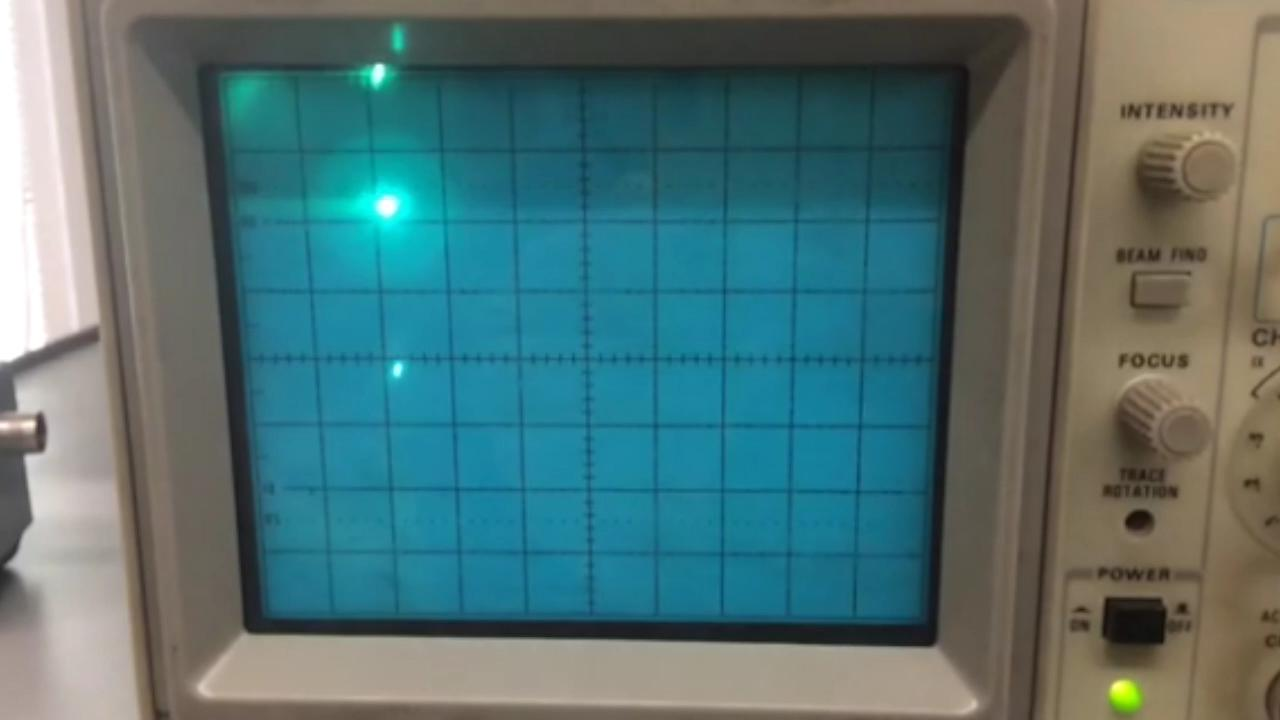
\includegraphics[scale = 0.08]{003.jpg}
    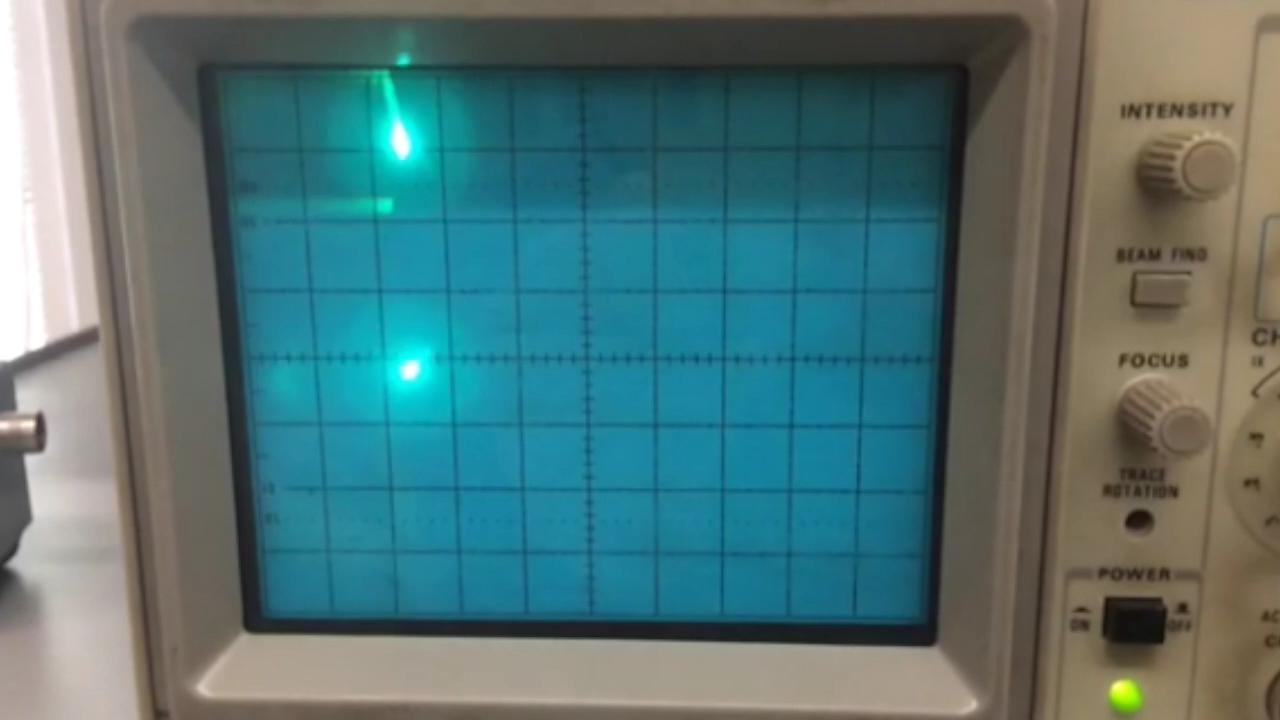
\includegraphics[scale = 0.08]{006.jpg}
    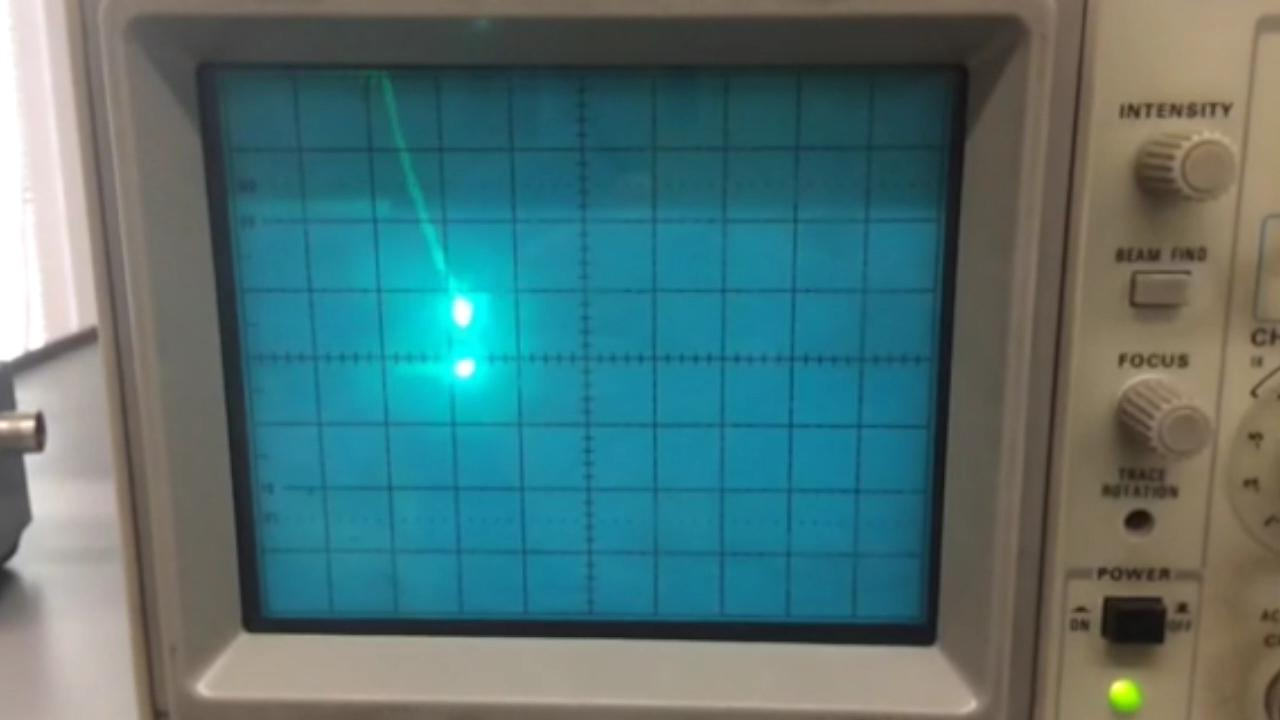
\includegraphics[scale = 0.08]{016.jpg}
    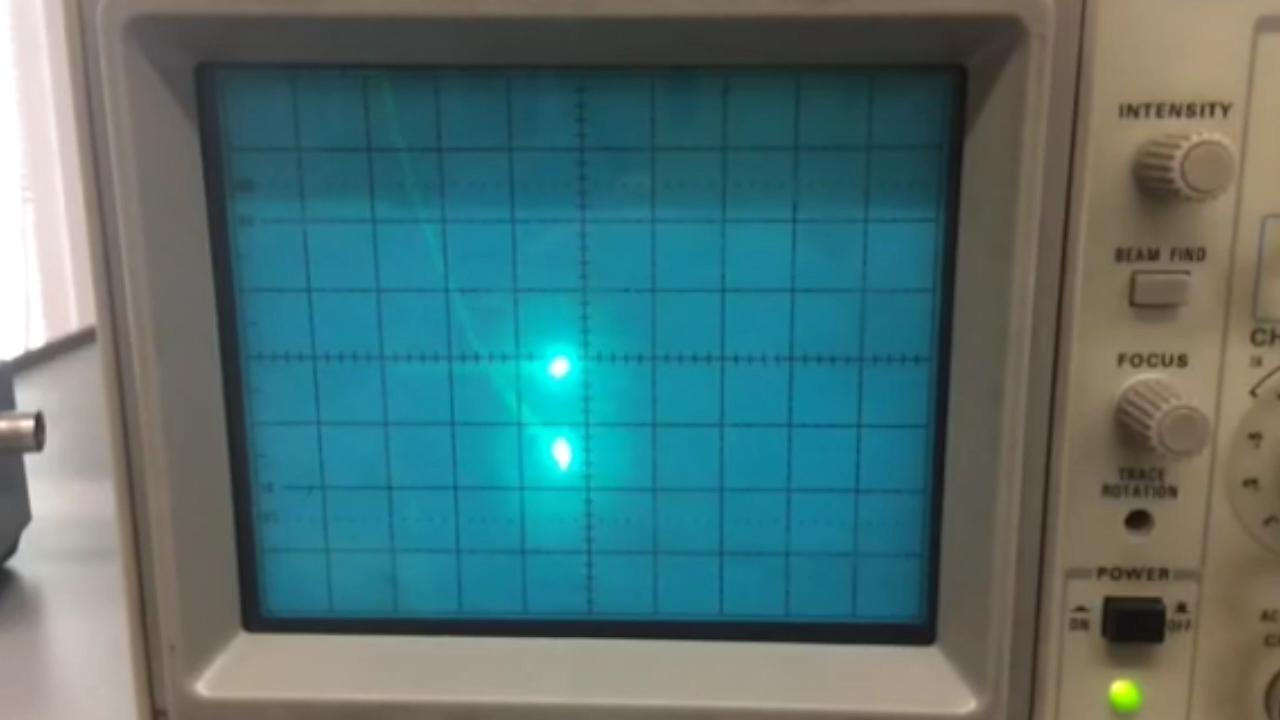
\includegraphics[scale = 0.08]{033.jpg}
    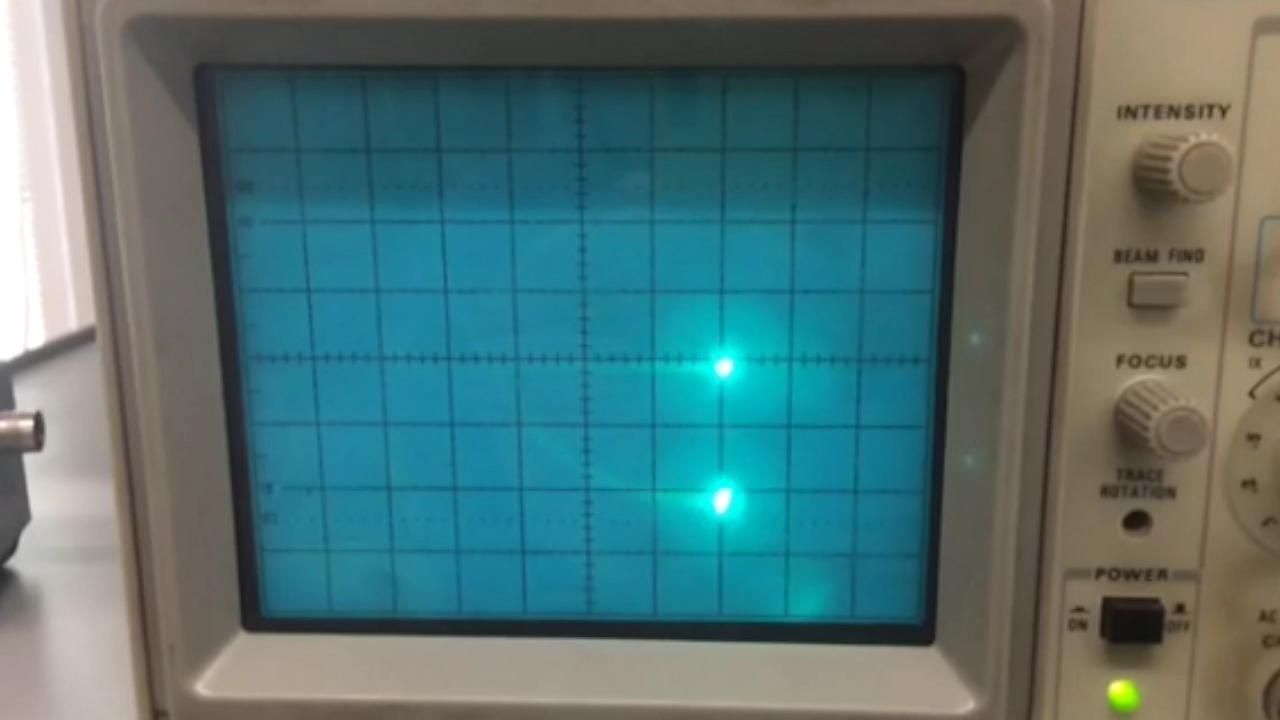
\includegraphics[scale = 0.08]{062.jpg}
    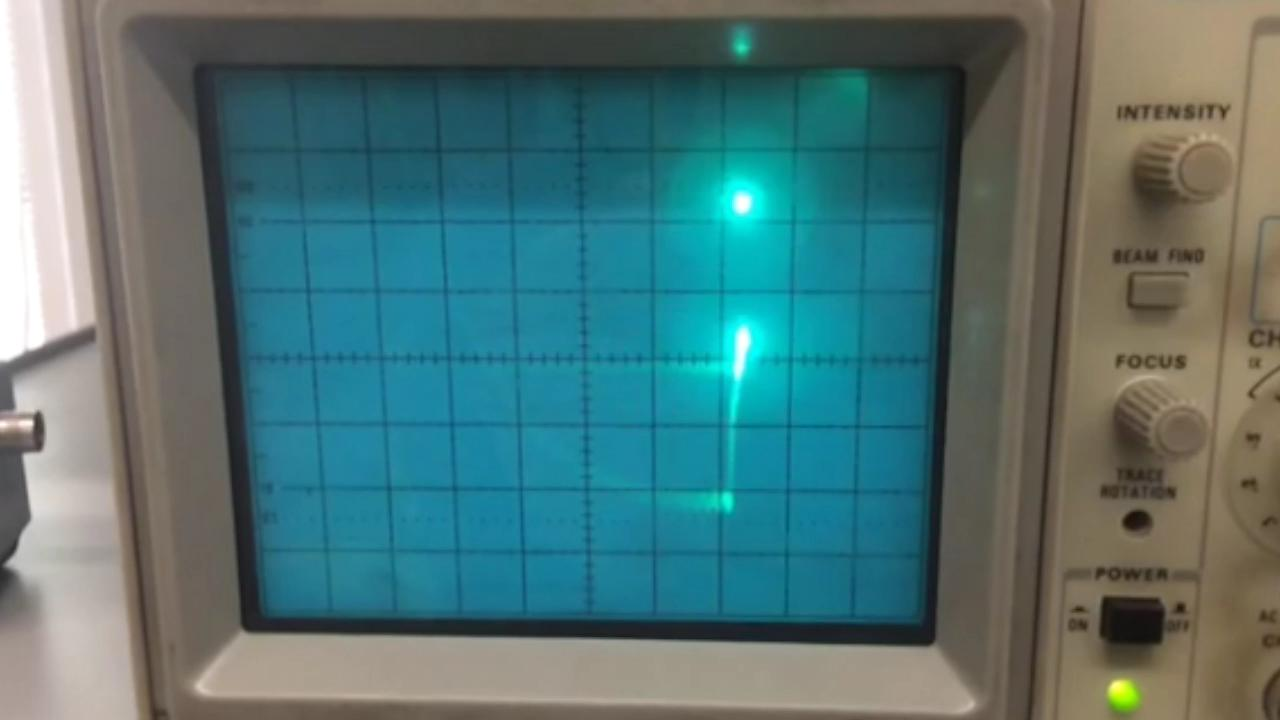
\includegraphics[scale = 0.08]{065.jpg}
    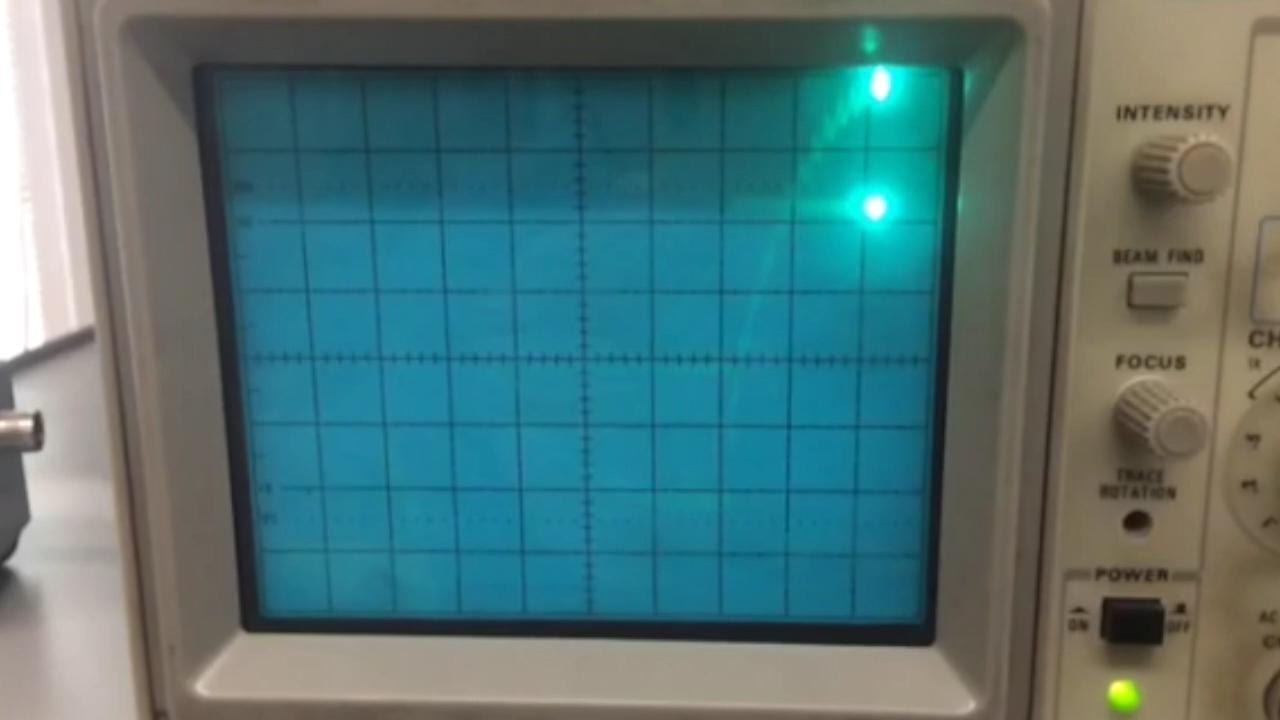
\includegraphics[scale = 0.08]{088.jpg}
    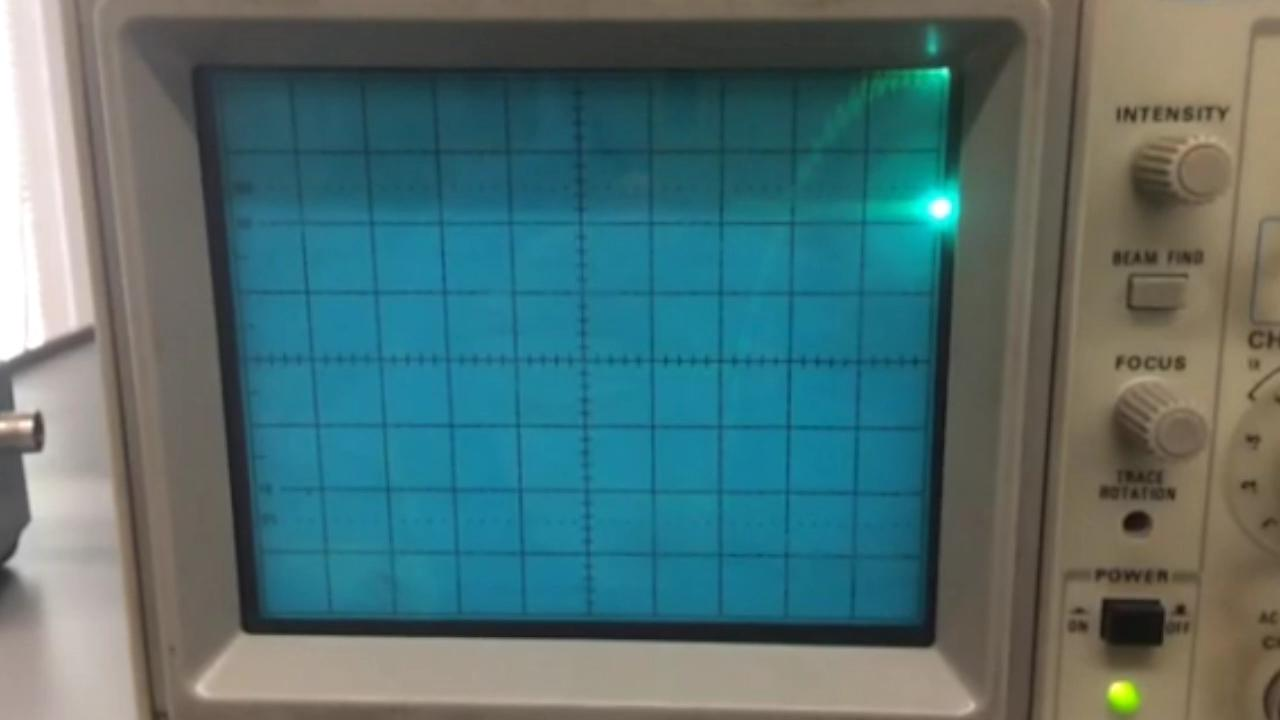
\includegraphics[scale = 0.08]{099.jpg}
    \caption{Selected Sample Images from High Speed Video Oscilloscope Output of Optical Pumping and Relaxation Processes of a Resonance Point of 85Rb}
    \label{fig:my_label}
\end{figure}

\begin{table}[H]
\centering
\caption{Pumping/Relaxation Time Data Points Cartesian Coordinates}
\label{my-label}
\scalebox{0.6}{
\begin{tabular}{llll}
\textbf{Pumping Time Data Points} & \textbf{(cartesian x,y)} & \textbf{Calibration Points} & \textbf{(x,y) Pixels} \\ \hline
\textbf{x Pixels} & \textbf{y Pixels} & $\vec{x_1}$ = & (374, 150) \\
378 & 72 & $\vec{x_2}$ = & (-586, 150) \\
394 & 112 & $\vec{x_3}$ = & (-384, 358) \\ \cline{3-4} 
428 & \multicolumn{1}{l|}{226} & \textbf{Relaxation Time} & \textbf{(x,y)} \\ \cline{3-4} 
458 & \multicolumn{1}{l|}{302} & \textbf{x Pixels} & \textbf{y Pixels} \\
488 & \multicolumn{1}{l|}{360} & 724 & 500 \\
518 & \multicolumn{1}{l|}{408} & 744 & 338 \\
546 & \multicolumn{1}{l|}{438} & 772 & 258 \\
576 & \multicolumn{1}{l|}{460} & 806 & 170 \\
602 & \multicolumn{1}{l|}{478} & 836 & 130 \\
630 & \multicolumn{1}{l|}{490} & 866 & 84 \\
658 & \multicolumn{1}{l|}{496} & 896 & 76 \\
686 & \multicolumn{1}{l|}{500} & 924 & 68 \\
712 & 500 &  &  \\
724 & 500 &  & 
\end{tabular}}
\end{table}





\end{document}

\begin{figure}[H] %FIX
    \centering
    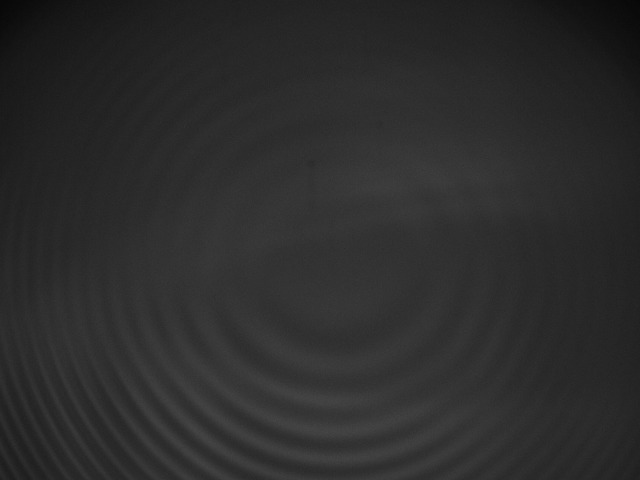
\includegraphics[scale = 0.1]{0.jpg}
    \caption{}
    \label{fig:my_label}
\end{figure}

sigfig, x equations, x cite, x format tables, x x label table and figures